%!TEX root = ../presentation.tex


\section{Bonnes pratiques des composantes \& BOM}

\subsection{Footprints}
\begin{frame}{Fabrication du footprint}
    \begin{twocolumns}
        \leftcol
        \begin{itemize}
            \item Élément très important de la conception de pièces
            \item Affecte le layout et l'assemblage
            \bigskip
            \item Le footprint devrait être clair
            \item Le footprint devrait être représentatif
            \item Le footprint devrait avoir des bonnes informations mécaniques
            \item Le footprint devrait respecter tes capacités d'assemblage
            \item Le footprint devrait avoir un modèle 3D
        \end{itemize}

        \rightcol
        \begin{itemize}
            \item Faire le footprint soi-même
            \begin{itemize}
                \item Suivre un standard
                \item Modifier la pièce plus tard au besoin
                \item Avoir des marqueurs de pin 1 consistants
                \item Avoir les bonnes couches mécaniques
                \item Avoir des bons modèles 3D
                \item Valider que le footprint est bon
            \end{itemize}
        \end{itemize}
    \end{twocolumns}
\end{frame}

\begin{frame}{Attention aux footprints!}
    \begin{twocolumns}
        \leftcol
        \begin{itemize}
            \item Toujours valider tous les footprints
            \item Faire attention aux sources de footprints
            \item Faire attention particulière aux transistors!
            \bigskip
            \item La meilleure option est de faire le footprint
        \end{itemize}
        \rightcol
        \makefigure[1][0.25][Microchip LND150]{transistor-lnd150-sgd}
        \makefigure[1][0.25][Vishay SQ2318]{transistor-sq2318-dgs}
    \end{twocolumns}
\end{frame}

\begin{frame}{Marqueurs de pin 1}
    \begin{twocolumns}
        \leftcol
        \only<1-2>{
            \begin{itemize}
                \item Doit être visible clairement pendant l'assemblage
                \begin{itemize}
                    \item Couche d'assemblage avec les marqueurs
                \end{itemize}
                \item Doit être visible après l'assemblage!
                \item Plusieurs marqueurs possibles
                \bigskip
                \item En vue 3D, il faut pouvoir immédiatement le voir
                \item Ne pas couvrir avec un via ou d'autre silkscreen!
            \end{itemize}
        }
        \only<3->{
            \makefigureborder[0.75][0.7]{footprint-qfn32-5x5}
        }
        \rightcol
        \only<1-2>{
            \tcbox[colframe=accent, colback=background]{
                \begin{tikzpicture}
                    \node[anchor=south west, inner sep=0] at (0,0) {
                        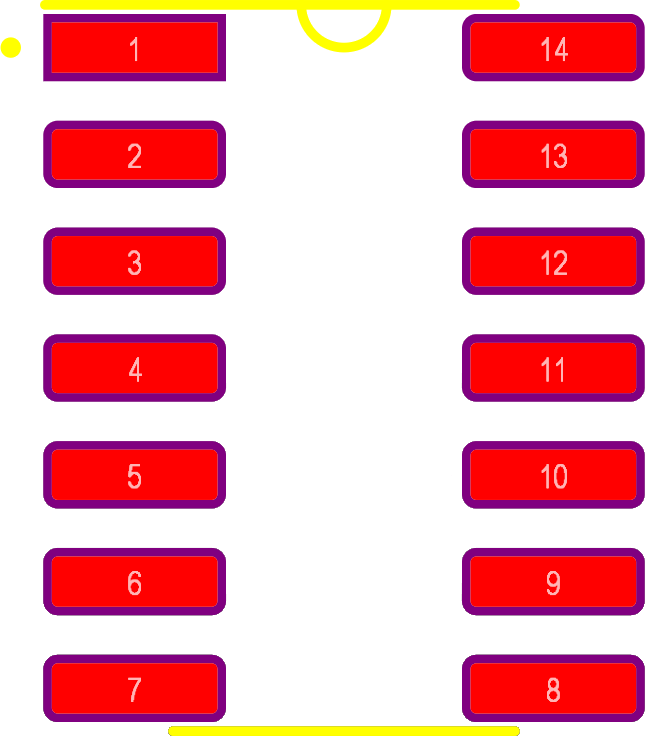
\includegraphics[width=0.75\textwidth,
                                         height=0.7\textheight,
                                         keepaspectratio]{
                            pictures/footprint-soic14-3_8mm}};
                    \only<2>{
                        \draw[accent, ultra thick, rounded corners] (-0.15, 5.35) rectangle (0.3, 5.8);
                        \draw[accent, ultra thick, rounded corners] (0.3, 5.8) rectangle (2, 6.1);
                        \draw[accent, ultra thick, rounded corners] (2.25, 5.35) rectangle (3.35, 6.1);
                        \draw[accent, ultra thick, rounded corners] (1.5, 5.25) rectangle (2, 5.5);
                    }
                \end{tikzpicture}
            }
        }
        \only<3->{
            \makefigureborder[0.75][0.7]{footprint-tssop20-4_4mm}
            }
    \end{twocolumns}
\end{frame}

% TODO: Couches mécaniques
% TODO: Vues 3D des pièces avec les marqueurs de pin #1
% S'assurer de respecter les couches mécaniques

\subsection{Symboles}

\begin{frame}{Fabrication du symbole}
    \begin{twocolumns}[0.6]
        \leftcol
        \begin{itemize}
            \item Un des éléments de clareté les plus importants
            \item Affecte aussi le BOM
            \bigskip
            \item La pièce devrait être représentative
            \item La pièce devrait être facile à lire
            \item La pièce devrait contenir toutes les informations pour le BOM
            \bigskip
            \item Faire la pièce soi-même
            \begin{itemize}
                \item Suivre un standard
                \item Modifier plus tard pour fitter le schéma
                \item Customize le BOM
                \item Validation de la pièce
                \item Mettre les types électriques
            \end{itemize}
        \end{itemize}

        \rightcol
        \makefigure[1][0.8][Source: \cite{kicad-symbol}]{kicad-pin-electrical-type}
    \end{twocolumns}
\end{frame}

\begin{frame}{Pinout du symbole}
    \begin{itemize}
        \item Garder les inputs à gauche et outputs à droite
        \item Ne pas numéroter le symbole comme le footprint
        \item Utiliser des symboles représentatifs lorsque possible
        \item Tu ne devrais pas avoir à aller dans la datasheet pour comprendre la pièce
    \end{itemize}
    \vfill
    \only<2-> {
    \begin{columns}
        \only<2> {
        \begin{column}{\textwidth}
        }
        \only<3> {
        \begin{column}{0.5\textwidth}
        }
        \only<4-> {
        \begin{column}{0.3\textwidth}
        }
            \begin{maketikzfigure}[1][0.4]
                \only<1-4>{
                \draw (0, 0) node
                   [dipchip,
                    num pins = 8,
                    %hide numbers,
                    external pins width=0.3,
                    external pad fraction=4,
                    anchor=bpin 1,
                    thick](op){\scriptsize OPA1632};
                }
                \only<5->{
                \draw (0, 0) node
                   [dipchip,
                    num pins = 8,
                    %hide numbers,
                    external pins width=0.3,
                    external pad fraction=4,
                    anchor=bpin 1,
                    thick, color=red](op){\scriptsize OPA1632};
                }
                \node [left,  font=\tiny] at (op.pin 1) {$V_{IN_-}$};
                \node [left,  font=\tiny] at (op.pin 2) {$V_{OCM}$};
                \node [left,  font=\tiny] at (op.pin 3) {$V_+$};
                \node [left,  font=\tiny] at (op.pin 4) {$V_{OUT_+}$};
                \node [right, font=\tiny] at (op.pin 5) {$V_{OUT_-}$};
                \node [right, font=\tiny] at (op.pin 6) {$V_-$};
                \node [right, font=\tiny] at (op.pin 7) {$EN$};
                \node [right, font=\tiny] at (op.pin 8) {$V_{IN_+}$};
            \end{maketikzfigure}
            \only<5-> {
                \begin{center}
                    \textcolor{red}{\textbf{BAD}}
                \end{center}
            }
        \end{column}

        \only<3> {
        \begin{column}{0.5\textwidth}
        }
        \only<4-> {
        \begin{column}{0.3\textwidth}
        }
        \only<3-> {
            \begin{maketikzfigure}[1][0.4]
                \only<1-4>{
                \draw (0, 0) node
                   [dipchip,
                    num pins = 8,
                    hide numbers,
                    external pins width=0.3,
                    external pad fraction=4,
                    anchor=bpin 1,
                    thick](op){\scriptsize OPA1632};
                }
                \only<5->{
                \draw (0, 0) node
                   [dipchip,
                    num pins = 8,
                    hide numbers,
                    external pins width=0.3,
                    external pad fraction=4,
                    anchor=bpin 1,
                    thick, color=blue](op){\scriptsize OPA1632};
                }
                \node [left,  font=\tiny] at (op.pin 1) {$V_{OCM}$};
                \node [right, font=\tiny] at (op.bpin 1) {$2$};
                \node [left,  font=\tiny] at (op.pin 2) {$V_{IN_+}$};
                \node [right, font=\tiny] at (op.bpin 2) {$8$};
                \node [left,  font=\tiny] at (op.pin 3) {$V_{IN_-}$};
                \node [right, font=\tiny] at (op.bpin 3) {$1$};
                \node [left,  font=\tiny] at (op.pin 4) {$EN$};
                \node [right, font=\tiny] at (op.bpin 4) {$7$};
                \node [right, font=\tiny] at (op.pin 5) {$V_-$};
                \node [left,  font=\tiny] at (op.bpin 5) {$6$};
                \node [right, font=\tiny] at (op.pin 6) {$V_{OUT_-}$};
                \node [left,  font=\tiny] at (op.bpin 6) {$5$};
                \node [right, font=\tiny] at (op.pin 7) {$V_{OUT_+}$};
                \node [left,  font=\tiny] at (op.bpin 7) {$4$};
                \node [right, font=\tiny] at (op.pin 8) {$V_+$};
                \node [left,  font=\tiny] at (op.bpin 8) {$3$};
            \end{maketikzfigure}
            \only<5-> {
                \begin{center}
                    \textcolor{blue}{\textbf{GOOD}}
                \end{center}
            }
        \end{column}
        }

        \only<4-> {
        \begin{column}{0.4\textwidth}
            \begin{maketikzfigure}[1][0.4]
                \only<1-4>{
                \draw (0, 0) node[fd op amp,
                                  thick, font=\normalsize,
                                  xscale=2, yscale=2,
                                  component text=left](op){\tiny OPA1632};
                }
                \only<5->{
                \draw (0, 0) node[fd op amp,
                                  thick, font=\normalsize,
                                  xscale=2, yscale=2,
                                  component text=left, color=accent](op){\tiny OPA1632};
                }
                \node[left,  font=\normalsize, label =15:{\scriptsize 8}] at (op.+)       {$V_{IN_+}$};
                \node[left,  font=\normalsize, label =15:{\scriptsize 1}] at (op.-)       {$V_{IN_-}$};
                \node[right, font=\normalsize, label=195:{\scriptsize 5}] at (op.out -)   {$V_{OUT_-}$};
                \node[right, font=\normalsize, label=165:{\scriptsize 4}] at (op.out +)   {$V_{OUT_+}$};
                \node[left,  font=\normalsize, label =15:{\scriptsize 2}] at (-2.4, 0)    {$V_{OCM}$};
                \node[left,  font=\normalsize, label =15:{\scriptsize 2}] at (-2.4, -2.4) {$EN$};

                \only<1-4>{
                    \draw[thick]
                    (-2.4, 0) to [short] (op.leftedge)
                    (op.up)   to (op.up   |- 0, 2)  node[vcc, font=\normalsize, label=285:{\scriptsize 3}] {$V_+$}
                    (op.down) to (op.down |- 0, -2) node[vee, font=\normalsize, label=105:{\scriptsize 6}] {$V_-$}
                    (-2.4, -2.4) to [short] (-1, -2.4) to [short] (-1, -1.6)
                    ;
                }
                \only<5->{
                    \draw[thick, color=accent]
                    (-2.4, 0) to [short] (op.leftedge)
                    (op.up)   to (op.up   |- 0, 2)  node[vcc, font=\normalsize, label=285:{\scriptsize 3}] {$V_+$}
                    (op.down) to (op.down |- 0, -2) node[vee, font=\normalsize, label=105:{\scriptsize 6}] {$V_-$}
                    (-2.4, -2.4) to [short] (-1, -2.4) to [short] (-1, -1.6)
                    ;
                }
            \end{maketikzfigure}
            \only<5-> {
                \begin{center}
                    \textcolor{accent}{\textbf{BEST}}
                \end{center}
            }
        \end{column}
        }
    \end{columns}
    }
\end{frame}

\begin{frame}{Symboles représentatifs}
    \begin{columns}
        \only<1>{
        \begin{column}{\textwidth}
        }
        \only<2->{
        \begin{column}{0.5\textwidth}
        }

        \only<1-2>{
            \begin{maketikzfigure}[1][0.8]
                \draw
                (0, 0) to [short, l={$ENABLE$}] (2, 0) to [R] (4, 0)
                to [full led, color=accent] (6, 0);
                \draw
                (0, -2) to [short, l={$POWER GOOD$}] (2, -2) to [R] (4, -2)
                to [full led, color=accent] (6, -2);
                \draw
                (0, -4) to [short, l={$STATUS$}] (2, -4) to [R] (4, -4)
                to [full led, color=red] (6, -4);
                \draw
                (0, -6) to [short, l={$HEARTBEAT$}] (2, -6) to [R] (4, -6)
                to [full led, color=orange] (6, -6);
                \draw
                (6, 0) to [short] (6, -7) node[ground, xscale=2, yscale=2]{};
            \end{maketikzfigure}
        }


        \only<3-4>{
            \ctikzset{multipoles/dipchip/width=2}
            \ctikzset{diodes/scale=0.5}
            \begin{maketikzfigure}[1][0.8]
                \draw (0, 0) node
                   [dipchip,
                    num pins = 12,
                    hide numbers, no topmark,
                    external pins width=0.3,
                    external pad fraction=4,
                    draw only pins={1, 3-4, 6}](esd){};
                \node at ($(esd.bpin 1) + (0.825, 0.4)$) {\tiny EPD2E001DRLR};

                \node [right, font=\tiny] at (esd.bpin 1) {$VCC$};
                \node [left,  font=\tiny] at (esd.pin  1) {$1$};
                \node [right, font=\tiny] at (esd.bpin 3) {$IO1$};
                \node [left,  font=\tiny] at (esd.pin  3) {$3$};
                \node [right, font=\tiny] at (esd.bpin 4) {$IO2$};
                \node [left,  font=\tiny] at (esd.pin  4) {$5$};
                \node [right, font=\tiny] at (esd.bpin 6) {$GND$};
                \node [left,  font=\tiny] at (esd.pin  6) {$4$};


                \draw ($(esd.bpin 1) + (0.65, 0)$) to ($(esd.bpin 1) + (2.25, 0)$);
                \draw ($(esd.bpin 3) + (0.5,  0)$) to ($(esd.bpin 3) + (1, 0)$);
                \draw ($(esd.bpin 4) + (0.5,  0)$) to ($(esd.bpin 4) + (1.75, 0)$);
                \draw ($(esd.bpin 6) + (0.65, 0)$) to ($(esd.bpin 6) + (2.25, 0)$);

                \draw ($(esd.bpin 3) + (1, 0)$) to
                      [full diode] ($(esd.bpin 1) + (1, 0)$);
                \draw ($(esd.bpin 4) + (1.75, 0)$) to
                      [short] ($(esd.bpin 3) + (1.75, 0)$) to
                      [full diode] ($(esd.bpin 1) + (1.75, 0)$);

                \draw ($(esd.bpin 6) + (1, 0)$) to 
                      [full diode] ($(esd.bpin 4) + (1, 0)$) to
                      [short] ($(esd.bpin 3) + (1, 0)$);
                \draw ($(esd.bpin 6) + (1.75, 0)$) to 
                      [full diode] ($(esd.bpin 4) + (1.75, 0)$);

                \draw ($(esd.bpin 6) + (2.25, 0)$) to
                      [full ZZener diode] ($(esd.bpin 1) + (2.25, 0)$);
            \end{maketikzfigure}
        }
        \only<5->{
            \ctikzset{multipoles/dipchip/width=2}
            \begin{maketikzfigure}[1][0.8]
                \draw (0, 0) node
                   [dipchip,
                    num pins = 12,
                    hide numbers, no topmark,
                    external pins width=0.3,
                    external pad fraction=4,
                    draw only pins={1, 3, 5-6, 7-8, 10, 12}](reg){};
            \node at ($(reg.bpin 1) + (0.825, 0.4)$) {\tiny LMZ23605TZE};

            \node [right, font=\tiny] at (reg.bpin 1) {$V_{IN}$};
            \node [left,  font=\tiny] at (reg.pin  1) {$1$};
            \node [right, font=\tiny] at (reg.bpin 3) {$EN$};
            \node [left,  font=\tiny] at (reg.pin  3) {$3$};
            \node [right, font=\tiny] at (reg.bpin 5) {$SYNC$};
            \node [left,  font=\tiny] at (reg.pin  5) {$2$};
            \node [right, font=\tiny] at (reg.bpin 6) {$SS$};
            \node [left,  font=\tiny] at (reg.pin  6) {$6$};

            \node [left,  font=\tiny] at (reg.bpin 7)  {$PGND$};
            \node [right, font=\tiny] at (reg.pin  7)  {$8$};
            \node [left,  font=\tiny] at (reg.bpin 8)  {$AGND$};
            \node [right, font=\tiny] at (reg.pin  8)  {$4$};
            \node [left,  font=\tiny] at (reg.bpin 10) {$FB$};
            \node [right, font=\tiny] at (reg.pin  10) {$5$};
            \node [left,  font=\tiny] at (reg.bpin 12) {$V_{OUT}$};
            \node [right, font=\tiny] at (reg.pin  12) {$7$};

            \end{maketikzfigure}
        }
        \end{column}

        \only<2-3>{
        \begin{column}{0.5\textwidth}
            \ctikzset{multipoles/dipchip/width=5}
            \begin{maketikzfigure}[1][0.8]
                \draw (0, 0) node
                   [dipchip,
                    num pins = 40,
                    hide numbers, no topmark,
                    external pins width=0.3,
                    external pad fraction=4,
                    draw only pins={1, 2, 4-5, 10, 11, 17, 18, 20, 21-22, 24-25, 27-28, 30-31, 33-34, 36-37, 39-40},
                    thick](adc){};
                \node at ($(adc.bpin 1) + (1.65, 0.5)$) {\textbf{ADS62P48IRGCT}};

                \node [right] at (adc.bpin 1) {$DVDD$};
                \node [left]  at (adc.pin  1) {$1$};
                \node [right] at (adc.bpin 2) {$AVDD$};
                \node [left]  at (adc.pin  2) {$16$};

                \node [right] at (adc.bpin 4) {$CLK_+$};
                \node [left]  at (adc.pin  4) {$25$};
                \node [right] at (adc.bpin 5) {$CLK_-$};
                \node [left]  at (adc.pin  5) {$26$};

                \node [right] at (adc.bpin 10) {$IN_+$};
                \node [left]  at (adc.pin  10) {$19$};
                \node [right] at (adc.bpin 11) {$IN_-$};
                \node [left]  at (adc.pin  11) {$20$};

                \node [right] at (adc.bpin 17) {$EN$};
                \node [left]  at (adc.pin  17) {$12$};
                \node [right] at (adc.bpin 18) {$RST$};
                \node [left]  at (adc.pin  18) {$15$};
                \node [right] at (adc.bpin 20) {$GND$};
                \node [left]  at (adc.pin  20) {$17$};

                \node [left]  at (adc.bpin 40) {$D0_+$};
                \node [right] at (adc.pin  40) {$61$};
                \node [left]  at (adc.bpin 39) {$D0_-$};
                \node [right] at (adc.pin  39) {$60$};
                \node [left]  at (adc.bpin 37) {$D1_+$};
                \node [right] at (adc.pin  37) {$63$};
                \node [left]  at (adc.bpin 36) {$D1_-$};
                \node [right] at (adc.pin  36) {$62$};
                \node [left]  at (adc.bpin 34) {$D2_+$};
                \node [right] at (adc.pin  34) {$3$};
                \node [left]  at (adc.bpin 33) {$D2_-$};
                \node [right] at (adc.pin  33) {$2$};
                \node [left]  at (adc.bpin 31) {$D3_+$};
                \node [right] at (adc.pin  31) {$5$};
                \node [left]  at (adc.bpin 30) {$D3_-$};
                \node [right] at (adc.pin  30) {$4$};
                \node [left]  at (adc.bpin 28) {$D4_+$};
                \node [right] at (adc.pin  28) {$7$};
                \node [left]  at (adc.bpin 27) {$D4_-$};
                \node [right] at (adc.pin  27) {$6$};
                \node [left]  at (adc.bpin 25) {$D5_+$};
                \node [right] at (adc.pin  25) {$9$};
                \node [left]  at (adc.bpin 24) {$D5_-$};
                \node [right] at (adc.pin  24) {$8$};
                \node [left]  at (adc.bpin 22) {$D6_+$};
                \node [right] at (adc.pin  22) {$11$};
                \node [left]  at (adc.bpin 21) {$D6_-$};
                \node [right] at (adc.pin  21) {$10$};

                % ADC
                \draw (-2.5, 0) to (-1.5, 1) to (-0.5, 1) to (-0.5, -1) to (-1.5, -1) to (-2.5, 0);
                \draw (adc.bpin 10 -| -2.75, 0) to (adc.bpin 10 -| -2.225, 0);
                \draw (adc.bpin 11 -| -2.75, 0) to (adc.bpin 11 -| -2.225, 0);
                \node at (-1.5, 0) {ADC};

                % DIFFERENTIAL DRIVERS
                \draw ($(adc.bpin 40) + (-1.75, 0.15)$) to ($(adc.bpin 39) + (-1.75, -0.15)$)
                to ($(adc.bpin 40) - (adc.bpin 31) + (2.5, 0)$) to ($(adc.bpin 40) + (-1.75, 0.15)$)
                ($(adc.bpin 40) - (1.485, 0)$) to ($(adc.bpin 40) - (1, 0)$)
                ($(adc.bpin 39) - (1.485, 0)$) to ($(adc.bpin 39) - (1, 0)$);

                \draw ($(adc.bpin 37) + (-1.75, 0.15)$) to ($(adc.bpin 36) + (-1.75, -0.15)$)
                to ($(adc.bpin 37) - (adc.bpin 31) + (2.5, 0)$) to ($(adc.bpin 37) + (-1.75, 0.15)$)
                ($(adc.bpin 37) - (1.485, 0)$) to ($(adc.bpin 37) - (1, 0)$)
                ($(adc.bpin 36) - (1.485, 0)$) to ($(adc.bpin 36) - (1, 0)$);

                \draw ($(adc.bpin 34) + (-1.75, 0.15)$) to ($(adc.bpin 33) + (-1.75, -0.15)$)
                to ($(adc.bpin 34) - (adc.bpin 31) + (2.5, 0)$) to ($(adc.bpin 34) + (-1.75, 0.15)$)
                ($(adc.bpin 34) - (1.485, 0)$) to ($(adc.bpin 34) - (1, 0)$)
                ($(adc.bpin 33) - (1.485, 0)$) to ($(adc.bpin 33) - (1, 0)$);

                \draw ($(adc.bpin 31) + (-1.75, 0.15)$) to ($(adc.bpin 30) + (-1.75, -0.15)$)
                to (2.5, 0) to ($(adc.bpin 31) + (-1.75, 0.15)$)
                ($(adc.bpin 31) - (1.485, 0)$) to ($(adc.bpin 31) - (1, 0)$)
                ($(adc.bpin 30) - (1.485, 0)$) to ($(adc.bpin 30) - (1, 0)$);

                \draw ($(adc.bpin 28) + (-1.75, 0.15)$) to ($(adc.bpin 27) + (-1.75, -0.15)$)
                to ($(adc.bpin 28) - (adc.bpin 31) + (2.5, 0)$) to ($(adc.bpin 28) + (-1.75, 0.15)$)
                ($(adc.bpin 28) - (1.485, 0)$) to ($(adc.bpin 28) - (1, 0)$)
                ($(adc.bpin 27) - (1.485, 0)$) to ($(adc.bpin 27) - (1, 0)$);

                \draw ($(adc.bpin 25) + (-1.75, 0.15)$) to ($(adc.bpin 24) + (-1.75, -0.15)$)
                to ($(adc.bpin 25) - (adc.bpin 31) + (2.5, 0)$) to ($(adc.bpin 25) + (-1.75, 0.15)$)
                ($(adc.bpin 25) - (1.485, 0)$) to ($(adc.bpin 25) - (1, 0)$)
                ($(adc.bpin 24) - (1.485, 0)$) to ($(adc.bpin 24) - (1, 0)$);

                \draw ($(adc.bpin 22) + (-1.75, 0.15)$) to ($(adc.bpin 21) + (-1.75, -0.15)$)
                to ($(adc.bpin 22) - (adc.bpin 31) + (2.5, 0)$) to ($(adc.bpin 22) + (-1.75, 0.15)$)
                ($(adc.bpin 22) - (1.485, 0)$) to ($(adc.bpin 22) - (1, 0)$)
                ($(adc.bpin 21) - (1.485, 0)$) to ($(adc.bpin 21) - (1, 0)$);

                % BUS
                \draw[very thick]
                (-0.5, 0) to (1.75, 0)
                (1, 0) to ($(adc.bpin 40) - (adc.bpin 31) + (1, 0)$)
                (1, 0) to ($(adc.bpin 22) - (adc.bpin 31) + (1, 0)$)
                ($(adc.bpin 40) - (adc.bpin 31) + (1, 0)$) to ($(adc.bpin 40) - (adc.bpin 31) + (1.75, 0)$)
                ($(adc.bpin 37) - (adc.bpin 31) + (1, 0)$) to ($(adc.bpin 37) - (adc.bpin 31) + (1.75, 0)$)
                ($(adc.bpin 34) - (adc.bpin 31) + (1, 0)$) to ($(adc.bpin 34) - (adc.bpin 31) + (1.75, 0)$)
                ($(adc.bpin 28) - (adc.bpin 31) + (1, 0)$) to ($(adc.bpin 28) - (adc.bpin 31) + (1.75, 0)$)
                ($(adc.bpin 25) - (adc.bpin 31) + (1, 0)$) to ($(adc.bpin 25) - (adc.bpin 31) + (1.75, 0)$)
                ($(adc.bpin 22) - (adc.bpin 31) + (1, 0)$) to ($(adc.bpin 22) - (adc.bpin 31) + (1.75, 0)$);
            \end{maketikzfigure}
        \end{column}
        }
        \only<4->{
            \begin{column}{0.5\textwidth}
                \ctikzset{multipoles/dipchip/width=2}
                \ctikzset{bipoles/resistor/height=0.1}
                \ctikzset{bipoles/resistor/width=0.3}
                \tikzset{vcc/.style={shape=vcc,/tikz/circuitikz/bipoles/length=0.75cm}}
                \begin{maketikzfigure}[1][0.8]
                    \draw (0, 0) node
                       [dipchip,
                        num pins = 22,
                        hide numbers, no topmark,
                        external pins width=0.3,
                        external pad fraction=4,
                        draw only pins={1, 3-4, 6-8, 10-11, 14-21}](io){};
                \node at ($(io.bpin 1) + (0.825, 0.4)$) {\tiny TCA9555RTWR};

                \node [right, font=\tiny] at (io.bpin 1) {$V_{CC}$};
                \node [right, font=\tiny] at (io.bpin 3) {$SDA$};
                \node [right, font=\tiny] at (io.bpin 4) {$SCL$};
                \node [right, font=\tiny] at (io.bpin 6) {$A0$};
                \node [right, font=\tiny] at (io.bpin 7) {$A1$};
                \node [right, font=\tiny] at (io.bpin 8) {$A2$};
                \node [right, font=\tiny] at (io.bpin 10) {$GND$};
                \node [right, font=\tiny] at (io.bpin 11) {$PAD$};

                \node [left, font=\tiny] at (io.bpin 21) {$P0$};
                \node [left, font=\tiny] at (io.bpin 20) {$P1$};
                \node [left, font=\tiny] at (io.bpin 19) {$P2$};
                \node [left, font=\tiny] at (io.bpin 18) {$P3$};
                \node [left, font=\tiny] at (io.bpin 17) {$P4$};
                \node [left, font=\tiny] at (io.bpin 16) {$P5$};
                \node [left, font=\tiny] at (io.bpin 15) {$P6$};
                \node [left, font=\tiny] at (io.bpin 14) {$P7$};

                \draw[densely dashed] ($(io.bpin 14) - (0.5,  0)$) to
                                      ($(io.bpin 14) - (0.75, 0)$) to
                                      ($(io.bpin 21) - (0.75, 0)$) to
                                      ($(io.bpin 21) - (0.5,  0)$);

                \draw (0.25, 0) to [R, l={\tiny$100K$}] node[vcc] {} (0.25, 1);
                \node [font=\tiny] at (0, -0.33) {Pull-up (8x)};
                \end{maketikzfigure}
            \end{column}
        }
    \end{columns}
\end{frame}


\begin{frame}{Laisser l'espace pour les composantes passives}
    \begin{columns}
        \only<1-4, 7>{
        \only<1-4>{
        \begin{column}{\textwidth}
        }
        \only<5->{
        \begin{column}{0.4\textwidth}
        }
            \ctikzset{multipoles/dipchip/width=2.5}
            \ctikzset{bipoles/resistor/height=0.2}
            \ctikzset{bipoles/resistor/width=0.5}
            \ctikzset{bipoles/capacitor/height=0.5}
            \ctikzset{bipoles/capacitor/width=0.15}
            \begin{maketikzfigure}[1][0.8]
                \draw (0, 0) node
                   [dipchip,
                    num pins = 8,
                    hide numbers, no topmark,
                    external pins width=0.3,
                    external pad fraction=4](reg){};
            \node at ($(reg.bpin 1) + (1.2, 0.5)$) {LMZ23605TZE};

            \node [right] at (reg.bpin 1) {$V_{IN}$};
            \node [right] at (reg.bpin 2) {$EN$};
            \node [right] at (reg.bpin 3) {$SYNC$};
            \node [right] at (reg.bpin 4) {$SS$};

            \node [left] at (reg.bpin 5)  {$PGND$};
            \node [left] at (reg.bpin 6)  {$AGND$};
            \node [left] at (reg.bpin 7) {$FB$};
            \node [left] at (reg.bpin 8) {$V_{OUT}$};

            % Vin
            \only<2->{
                \draw (reg.pin 1) to [short] ($(reg.pin 1) - (4.5, 0)$)
                to [short]      ($(reg.pin 1) - (4.5, -0.25)$)
                to node[vcc] {} ($(reg.pin 1) - (4.5, -0.25)$);
            }

            % EN
            \only<2-3>{
                \draw (reg.pin 2) to [short] ($(reg.pin 2) - (2.5, 0)$)
                    to [R]     ($(reg.pin 2) - (4.5, 0)$)
                to [short] ($(reg.pin 1) - (4.5, -0.25)$)
                ($(reg.pin 2) - (2.5, 0)$) to [R] ($(reg.pin 4) - (2.5, 1.5)$)
                to node[ground]{} ($(reg.pin 4) - (2.5, 1.5)$);
            }
            \only<4->{
                \draw (reg.pin 2) to [short] ($(reg.pin 2) - (2.5, 0)$)
                    to [R, l2={$R_1$} and {$\SI{4.7}{\kilo\ohm}$},
                        a2={$0603$} and {$5\%$},
                        l2 halign=c, a2 halign=c,
                        label distance=-1pt, annotation distance=-56pt]
                    ($(reg.pin 2) - (4.5, 0)$)
                to [short] ($(reg.pin 1) - (4.5, -0.25)$)
                ($(reg.pin 2) - (2.5, 0)$)
                    to [R, l2={$R_2$} and {$\SI{10}{\kilo\ohm}$},
                        a2={$0603$} and {$5\%$},
                        l2 halign=c, a2 halign=c]
                    ($(reg.pin 4) - (2.5, 1.5)$)
                to node[ground]{} ($(reg.pin 4) - (2.5, 1.5)$);
            }


            % SS
            \only<2-3>{
                \draw (reg.pin 4) to [short] ($(reg.pin 4) - (0.5, 0)$)
                    to [C] ($(reg.pin 4) - (0.5, 1)$)
                    to node[ground]{} ($(reg.pin 4) - (0.5, 1.5)$);
            }
            \only<4->{
                \draw (reg.pin 4) to [short] ($(reg.pin 4) - (0.5, 0)$)
                    to [C, l2={$C_1$} and {$\SI{100}{\nano\farad}$},
                           a2={$0603$} and {$25V$},
                           l2 halign=c, a2 halign=c]
                        ($(reg.pin 4) - (0.5, 1)$)
                    to node[ground]{} ($(reg.pin 4) - (0.5, 1.5)$);
            }

            % SYNC
            \only<2-3>{
                \draw (reg.pin 3) to [short] ($(reg.pin 3) - (1.5, 0)$)
                    to [C] ($(reg.pin 4) - (1.5, 1)$)
                    to node[ground]{} ($(reg.pin 4) - (1.5, 1.5)$);
            }
            \only<4->{
                \draw (reg.pin 3) to [short] ($(reg.pin 3) - (1.5, 0)$)
                    to [C, l2={$C_1$} and {$\SI{100}{\nano\farad}$},
                           a2={$0603$} and {$25V$},
                           l2 halign=c, a2 halign=c]
                        ($(reg.pin 4) - (1.5, 1)$)
                    to node[ground]{} ($(reg.pin 4) - (1.5, 1.5)$);
            }

            % GND
            \only<2->{
                \draw (reg.pin 5) to [short] ($(reg.pin 5) + (1, 0)$)
                to [short] ($(reg.pin 5) + (1, -1.25)$)
                to node[ground]{} ($(reg.pin 5) + (1, -1.5)$);

            \draw (reg.pin 6) to [short] ($(reg.pin 6) + (1.25, 0)$)
            to ($(reg.pin 5) + (1.25, -1)$)
            to ($(reg.pin 5) + (1, -1)$);
            }

            % FB
            \only<2-3>{
                \draw (reg.pin 7) to [short] ($(reg.pin 7) + (2.5, 0)$)
                to [R]     ($(reg.pin 7) + (4.5, 0)$)
                to [short] ($(reg.pin 8) + (4.5, 0.25)$)
                ($(reg.pin 7) + (2.5, 0)$) to [R] ($(reg.pin 5) + (2.5, -1.5)$)
                to node[ground]{} ($(reg.pin 5) + (2.5, -1.5)$);
            }
            \only<4->{
                \draw (reg.pin 7) to [short] ($(reg.pin 7) + (2.5, 0)$)
                to [R, l2={$R_3$} and {$\SI{5.9}{\kilo\ohm}$},
                        a2={$0603$} and {$5\%$},
                        l2 halign=c, a2 halign=c,
                        label distance=-28pt, annotation distance=44pt]
                    ($(reg.pin 7) + (4.5, 0)$)
                to [short] ($(reg.pin 8) + (4.5, 0.25)$)
                ($(reg.pin 7) + (2.5, 0)$)
                to [R, l2={$R_4$} and {$\SI{10}{\kilo\ohm}$},
                        a2={$0603$} and {$5\%$},
                        l2 halign=c, a2 halign=c]
                    ($(reg.pin 5) + (2.5, -1.5)$)
                to node[ground]{} ($(reg.pin 5) + (2.5, -1.5)$);
            }

            % Vout
            \only<2->{
                \draw (reg.pin 8) to [short] ($(reg.pin 8) + (4.5, 0)$)
                to [short]      ($(reg.pin 8) + (4.5, 0.25)$)
                to node[vcc] {} ($(reg.pin 8) + (4.5, 0.25)$);
            }

            % Boxes
            \only<3> {
                \draw[dashed, thick, color=red]
                    ($(reg.pin 5) + (2.25, -2.1)$) to ($(reg.pin 4) - (2.25, 2.1)$);

                \draw[dashed, thick, rounded corners, color=red]
                    ($(reg.pin 2) - (4.25, -0.45)$) rectangle ($(reg.pin 2) - (2.75, 0.45)$);

                \draw[dashed, thick, rounded corners, color=red]
                    ($(reg.pin 7) + (4.25, 0.45)$) rectangle ($(reg.pin 7) + (2.75, -0.45)$);

                \draw[dashed, thick, rounded corners, color=red]
                    ($(reg.pin 3) - (2, 0.25)$) rectangle ($(reg.pin 4) - (-0.1, 1)$);

                \draw[dashed, thick, rounded corners, color=red]
                    ($(reg.pin 6) + (0.75, 0.15)$) rectangle ($(reg.pin 6) + (1.5, -1.65)$);
            }
            \end{maketikzfigure}
        \end{column}
        }

        \only<5->{
        \only<5-6>{
        \begin{column}{\textwidth}
        }
        \only<7->{
        \begin{column}{0.5\textwidth}
        }
            \ctikzset{multipoles/dipchip/width=2.5}
            \ctikzset{bipoles/resistor/height=0.2}
            \ctikzset{bipoles/resistor/width=0.5}
            \ctikzset{bipoles/capacitor/height=0.5}
            \ctikzset{bipoles/capacitor/width=0.15}
                \begin{maketikzfigure}[1][0.8]
                    \draw (0, 0) node
                       [dipchip,
                        num pins = 12,
                        hide numbers, no topmark,
                        external pins width=0.3,
                        external pad fraction=4,
                        draw only pins={1, 3, 5-6, 7-8, 10, 12}](reg){};
                \node at ($(reg.bpin 1) + (0.825, 0.4)$) {\tiny LMZ23605TZE};

                \node [right, font=\tiny] at (reg.bpin 1) {$V_{IN}$};
                \node [right, font=\tiny] at (reg.bpin 3) {$EN$};
                \node [right, font=\tiny] at (reg.bpin 5) {$SYNC$};
                \node [right, font=\tiny] at (reg.bpin 6) {$SS$};

                \node [left,  font=\tiny] at (reg.bpin 7)  {$PGND$};
                \node [left,  font=\tiny] at (reg.bpin 8)  {$AGND$};
                \node [left,  font=\tiny] at (reg.bpin 10) {$FB$};
                \node [left,  font=\tiny] at (reg.bpin 12) {$V_{OUT}$};

                % Vin
                \only<6->{
                \draw (reg.pin 1) to [short] ($(reg.pin 1) - (3.5, 0)$)
                to [short]      ($(reg.pin 1) - (3.5, -0.25)$)
                to node[vcc] {} ($(reg.pin 1) - (3.5, -0.25)$);
                }

                % EN
                \only<6->{
                    \draw (reg.pin 3) to [short] ($(reg.pin 3) - (3.5, 0)$)
                        to [R]     ($(reg.pin 1) - (3.5, 0)$)
                    to [short] ($(reg.pin 1) - (3.5, -0.25)$)
                    ($(reg.pin 3) - (3.5, 0)$) to [R] ($(reg.pin 6) - (3.5, 1.5)$)
                    to node[ground]{} ($(reg.pin 6) - (3.5, 2)$);
                }

                % SS
                \only<6->{
                    \draw (reg.pin 6) to [short] ($(reg.pin 6) - (0.5, 0)$)
                        to [C] ($(reg.pin 6) - (0.5, 1.5)$)
                        to node[ground]{} ($(reg.pin 6) - (0.5, 2)$);
                }

                % SYNC
                \only<6->{
                    \draw (reg.pin 5) to [short] ($(reg.pin 5) - (1.75, 0)$)
                        to [short] ($(reg.pin 6) - (1.75, 0)$)
                        to [C] ($(reg.pin 6) - (1.75, 1.5)$)
                        to node[ground]{} ($(reg.pin 6) - (1.75, 2)$);
                }


                % Vout
                \only<6->{
                \draw (reg.pin 12) to [short] ($(reg.pin 12) + (1.5, 0)$)
                to [short]      ($(reg.pin 12) + (1.5, 0.25)$)
                to node[vcc] {} ($(reg.pin 12) + (1.5, 0.25)$);
                }


                % FB
                \only<6->{
                    \draw (reg.pin 10) to [short] ($(reg.pin 10) + (1.5, 0)$)
                        to [R]     ($(reg.pin 12) + (1.5, 0)$)
                    to [short] ($(reg.pin 12) + (1.5, 0.25)$)
                    ($(reg.pin 10) + (1.5, 0)$) to [R] ($(reg.pin 7) + (1.5, -1.5)$)
                    to node[ground]{} ($(reg.pin 7) + (1.5, -2)$);
                }

                % GND
                \only<6->{
                    \draw (reg.pin 7) to [short] ($(reg.pin 7) + (0.5, 0)$);
                    \draw (reg.pin 8) to [short] ($(reg.pin 8) + (0.5, 0)$)
                        to ($(reg.pin 7) + (0.5, -1.5)$)
                        to node[ground]{} ($(reg.pin 7) + (0.5, -2)$);
                }

                % Text
                \only<6->{
                    \node at ($(reg.pin 6) - (-0.25, 1.25)$) {
                        \begin{minipage}{2cm}
                            \centering
                            \footnotesize
                            $C_2$\\
                            $\SI{100}{\nano\farad}$\\
                            $0603$\\
                            $\SI{50}{\volt}$
                        \end{minipage}
                    };
                    \node at ($(reg.pin 6) - (2.5, 1.25)$) {
                        \begin{minipage}{2cm}
                            \centering
                            \footnotesize
                            $C_1$\\
                            $\SI{100}{\nano\farad}$\\
                            $0603$\\
                            $\SI{50}{\volt}$
                        \end{minipage}
                    };
                    \node at ($(reg.pin 2) - (4.65, 0.1)$) {
                        \begin{minipage}{2cm}
                            \centering
                            \footnotesize
                            $R_1$\\
                            $\SI{4.7}{\kilo\ohm}$\\
                            $0603$\\
                            $5\%$
                        \end{minipage}
                    };
                    \node at ($(reg.pin 2) - (4.65, 2.25)$) {
                        \begin{minipage}{2cm}
                            \centering
                            \footnotesize
                            $R_2$\\
                            $\SI{10}{\kilo\ohm}$\\
                            $0603$\\
                            $5\%$
                        \end{minipage}
                    };
                    \node at ($(reg.pin 10) + (2.15, 0.5)$) {
                        \begin{minipage}{2cm}
                            \centering
                            \footnotesize
                            $R_3$\\
                            $\SI{5.9}{\kilo\ohm}$\\
                            $0603$\\
                            $5\%$
                        \end{minipage}
                    };
                    \node at ($(reg.pin 10) + (2.15, -1.75)$) {
                        \begin{minipage}{2cm}
                            \centering
                            \footnotesize
                            $R_4$\\
                            $\SI{10}{\kilo\ohm}$\\
                            $0603$\\
                            $5\%$
                        \end{minipage}
                    };
                }
                \end{maketikzfigure}
        \end{column}
        }
    \end{columns}
\end{frame}


\begin{frame}{Informations du BOM}
    \begin{itemize}
        \item Toujours mettre la datasheet dans la pièce
        \item Manufacturier et part number complet (ce qui va être commandé au final)
        \item Plages d'opérations (température, tension, courant)
        \item Fournisseurs (avec liens pour les achats)
        \item Qui a fait le symbole, qui l'a révisé et quand (suivi)
    \end{itemize}
    \makefigure[1][0.45]{kicad-symbol-parameters}
\end{frame}

\subsection{Datasheets}

\begin{frame}{Lecture de datasheets}
    \only<1-2>{
    \begin{twocolumns}[0.5]
    }
    \only<3->{
    \begin{twocolumns}[0.4]
    }
        \leftcol
        \begin{itemize}
            \item<1-> Toujours lire \href{https://ww1.microchip.com/downloads/aemDocuments/documents/APID/ProductDocuments/DataSheets/MCP3561_2_4R-Data-Sheet-DS200006391C.pdf}{la datasheet} au complet!
            \item<2-> Lire les schémas d'\textit{evaluation boards}
            \item<3-> Lire les application notes
        \end{itemize}

        \only<1>{
            \makefigure[1][0.45]{datasheet-mcp3561-block-diagram}
            \vfill
        }
        \only<2>{
            \vspace{-24pt}
            \makefigure[1][0.45]{datasheet-mcp3561-eval}
            \vfill
        }
        \rightcol
        % Datasheet
        \only<1>{
        \begin{itemize}
            \item \textbf{\textit{Absolute Maximum Ratings}}
            \item Toutes les \textit{Electrical Characteristics}
            \item \textbf{Spécifications et équations}
            \item \textbf{Description des pins}
            \item Graphiques (surtout les courbes de power)
            \item Overview des fonctionalités
            \item \textbf{Modes d'opérations}
            \item \textbf{Modes de configurations}
            \item Alimentation
            \item \textbf{Schémas et Layout recommandés}
            \item Registres
        \end{itemize}
        }
        % Evaluation Board
        \only<2>{
        \begin{itemize}
            \item Modes d'utilisation
            \item \textbf{Schémas}
            \item \textbf{Layout}
            \item Logiciel / Code / Firmware
            \item \textbf{BOM et choix de pièces}
            \item Calculs
        \end{itemize}
        }
        % Application Notes
        \only<3>{
        \begin{itemize}
            \item Modes d'utilisation
            \item Séquences d'alimentation
            \item Programmation
            \item Layouts spécifiques
            \item Calculs
        \end{itemize}
        }
        \only<4>{
        \footnotesize
        \begin{itemize}
            \item ECP5 and ECP5-5G Family Data Sheet
            \item ECP5 and ECP5-5G Hardware Checklist
            \item ECP5 and ECP5-5G High-Speed I/O Interface
            \item ECP5 and ECP5-5G Memory User Guide
            \item ECP5 and ECP5-5G SerDes/PCS Usage Guide
            \item ECP5 and ECP5-5G sysCLOCK PLL/DLL
            \item ECP5 and ECP5-5G sysIO Usage Guide
            \item ECP5 Automotive Family Data Sheet
            \item ECP5 Errata - SED Function with Distributed RAM
            \item Electrical Recommendations for Lattice SERDES
            \item PCB Layout Recommendations for BGA Packages
            \item Power Consumption and Management for ECP5 Devices
            \item Thermal Management for Lattice Devices
        \end{itemize}
        }
    \end{twocolumns}
\end{frame}

\begin{frame}{Configurateurs}
    \begin{twocolumns}
        \leftcol
        \begin{itemize}
            \item Manufacturier donne parfois des configurateurs
            \item Valider les calculs avec la datasheet
            \item Ne pas utiliser uniquement le configurateur!
            \item Donne aussi un BOM sur lequel se fier
        \end{itemize}
        \rightcol
        \makefigure{pllatinum}
    \end{twocolumns}
\end{frame}

\begin{frame}{Configurateurs (TI WeBench)}
    \makefigure[1][0.9]{webench}
\end{frame}

\begin{frame}{Plages et courbes}
    \begin{twocolumns}
        \leftcol
        \begin{itemize}
            \item Valider toutes les courbes au point d'opération
            \item Valider les plages d'opérations
            \begin{itemize}
                \item Sur toutes les IO
                \item Sur les alimentations
            \end{itemize}
        \end{itemize}
        \rightcol
        \begin{itemize}
            \item Valider les plages de tension
            \begin{itemize}
                \item Besoin d'un heatsink?
                \item Besoin de dissipation thermique?
                \item A quel point est-ce que ça va chauffer?
            \end{itemize}
        \end{itemize}
    \end{twocolumns}

    \makefigure[0.8][0.7]{datasheet-mcp3561-thermal}
\end{frame}

\begin{frame}{Passer au travers d'une datasheet}
    \begin{twocolumns}
        \leftcol
            \begin{center}
                \textbf{MCP3561}
            \end{center}
            \begin{itemize}
                \item ADC 24-bit
                \item Architecture Sigma-Delta
                \item 8 entrées multiplexées
                \item Gain programmable
                \item Capteur de température
                \item Interface SPI
                \item Programmable par registres internes
            \end{itemize}
        \rightcol
        \makefigure[0.66][0.5][https://www.microchip.com/en-us/product/mcp3561]{mcp3561-ic}
    \end{twocolumns}
\end{frame}

% TODO: Passer au travers d'une datasheet
% https://ww1.microchip.com/downloads/aemDocuments/documents/APID/ProductDocuments/DataSheets/MCP3561_2_4R-Data-Sheet-DS200006391C.pdf

\subsection{Recherche de pièces}

\begin{frame}
    \begin{tikzpicture}
        \node[anchor=south west, inner sep=0] at (0,0) {
            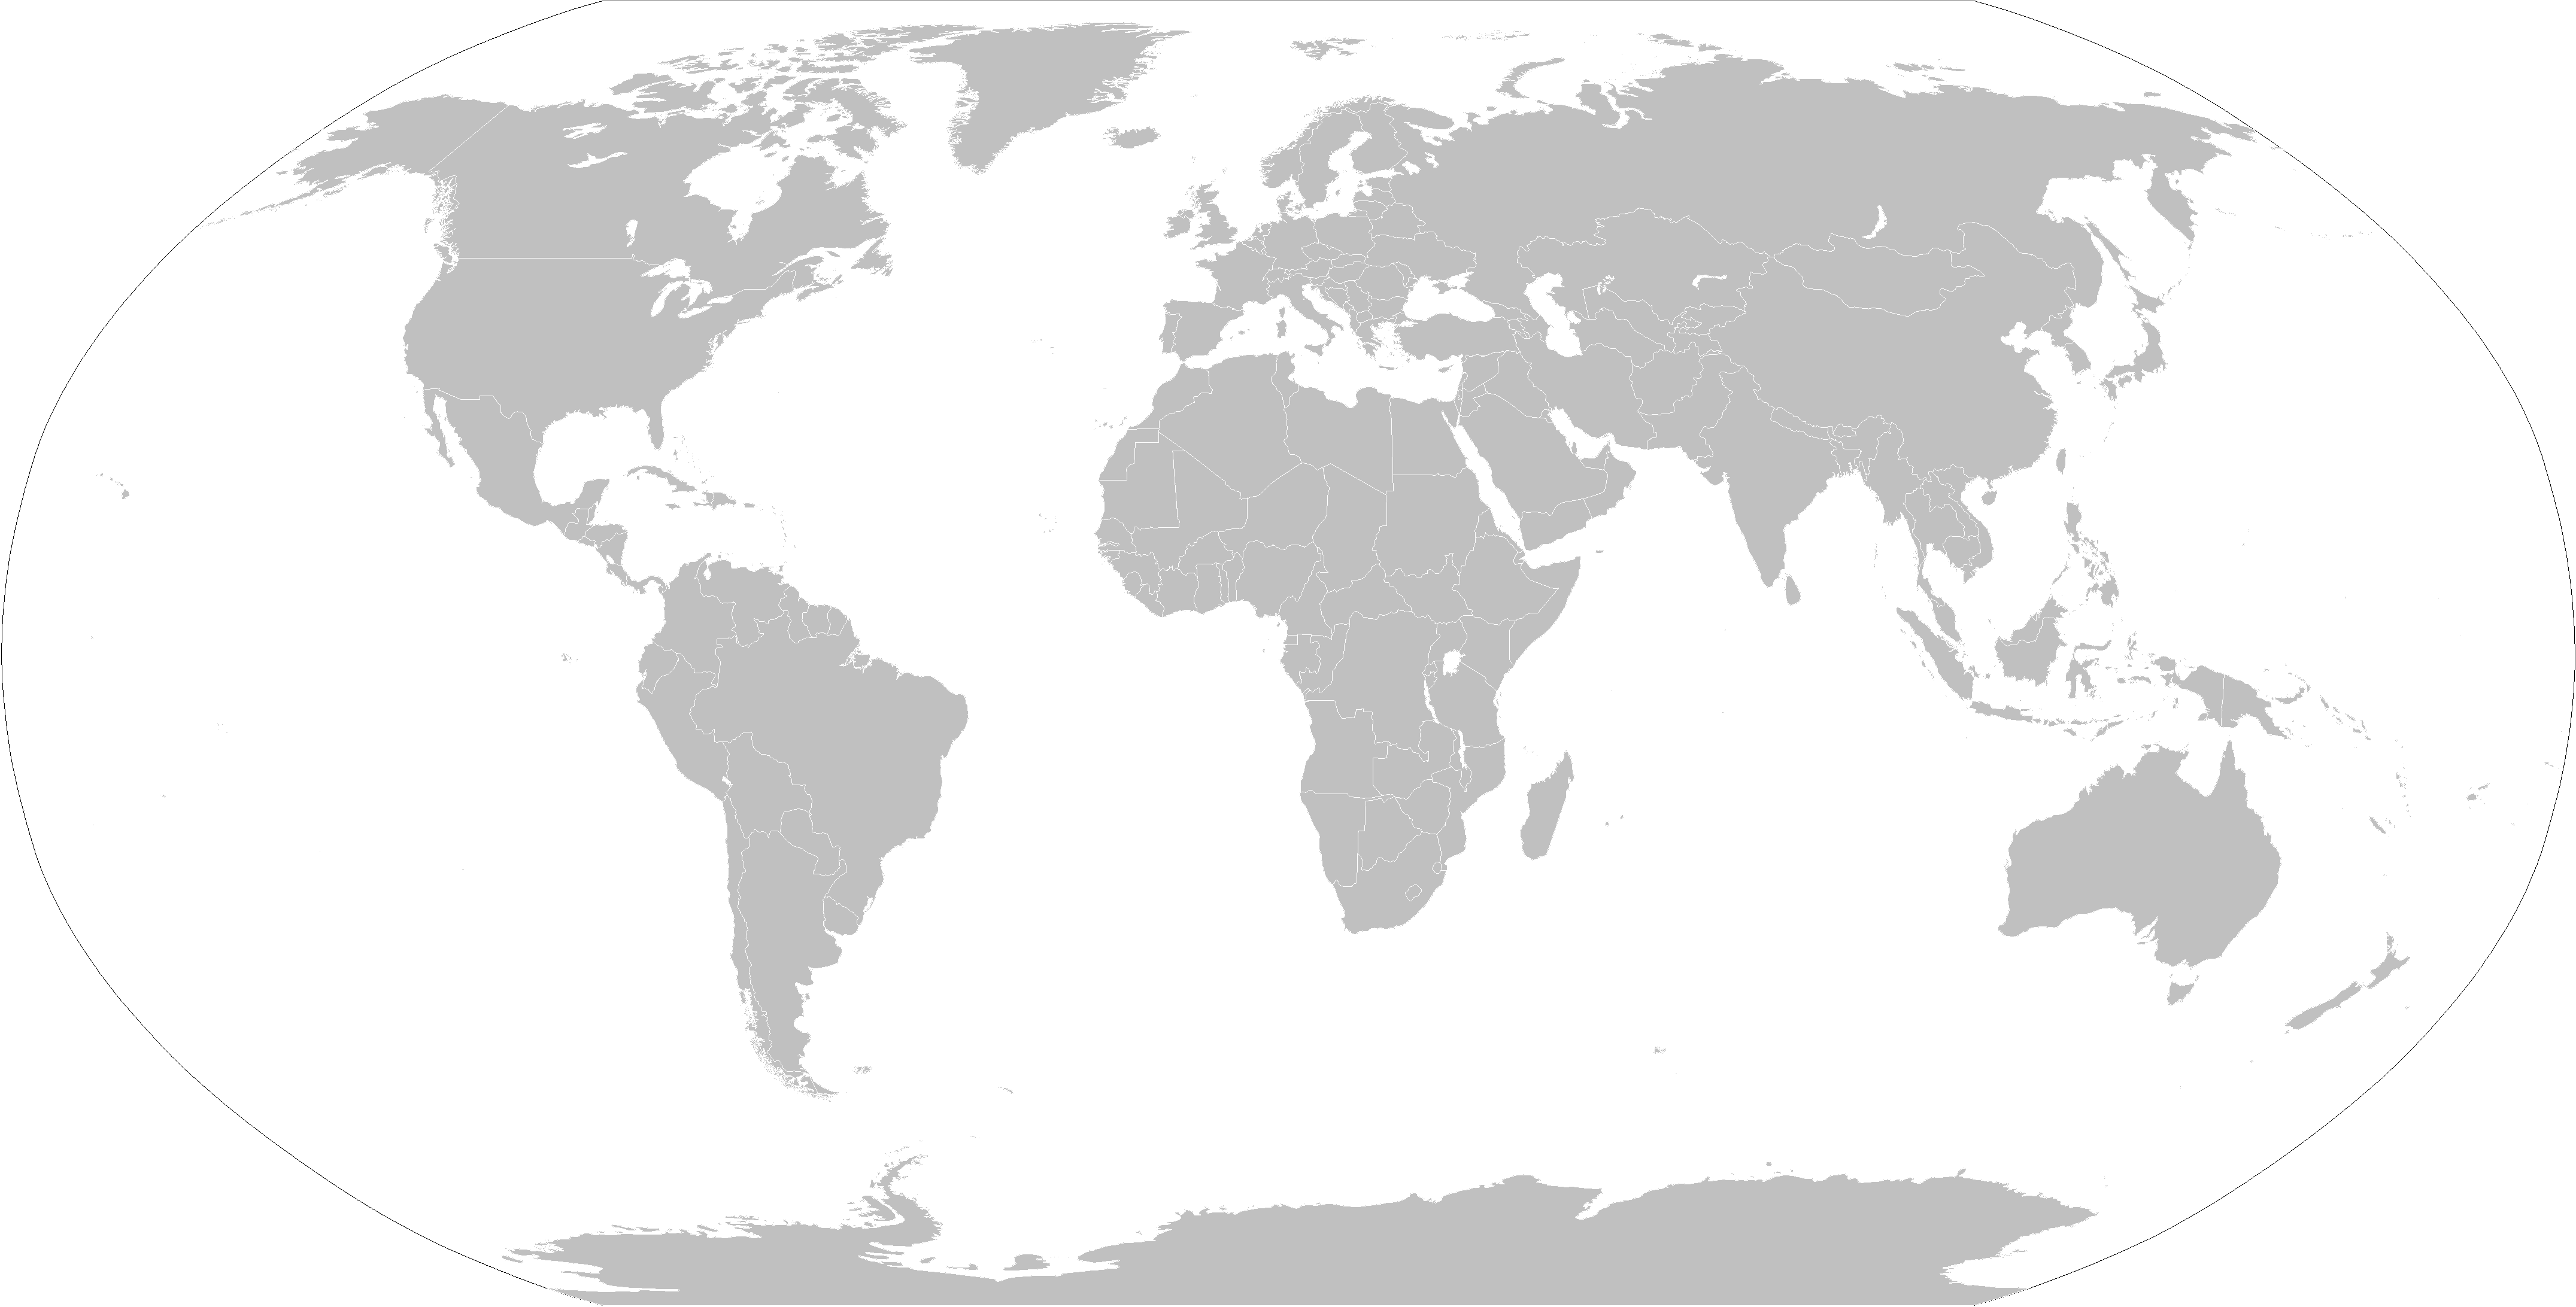
\includegraphics[width=\textwidth,
                             height=\textheight,
                             keepaspectratio]{
                pictures/world}};

        \node[color=accent] at (3.75, 6.25) {\faMapMarker*};
        \node[color=accent] at (3.75, 6.55) {
\includegraphics[width=0.045\textwidth,
                                                              height=0.045\textheight,
                                                              keepaspectratio]
                                                {pictures/distributors/digikey}};

        \node[color=accent] at (3, 5.8) {\faMapMarker*};
        \node[color=accent] at (3, 6.1) {
\includegraphics[width=0.04\textwidth,
                                                          height=0.04\textheight,
                                                          keepaspectratio]
                                                {pictures/distributors/arrow}};

        \node[color=accent] at (4.5, 6.25) {\faMapMarker*};
        \node[color=accent] at (4.5, 6.65)  {
\includegraphics[width=0.03\textwidth,
                                                              height=0.03\textheight,
                                                              keepaspectratio]
                                                {pictures/distributors/future-electronics}};

        \node[color=accent] at (11.825, 5.15) {\faMapMarker*};
        \node[color=accent] at (11.825, 5.55)  {
\includegraphics[width=0.03\textwidth,
                                                                 height=0.03\textheight,
                                                                 keepaspectratio]
                                                {pictures/distributors/lcsc}};

        \node[color=accent] at (3.4, 5.6)  {\faMapMarker*};
        \node[color=accent] at (3.4, 5.95) {
\includegraphics[width=0.03\textwidth,
                                                             height=0.03\textheight,
                                                             keepaspectratio]
                                                {pictures/distributors/mouser}};

        \node[color=accent] at (7.25, 6.6)  {\faMapMarker*};
        \node[color=accent] at (7.25, 6.95) {
\includegraphics[width=0.03\textwidth,
                                                             height=0.03\textheight,
                                                             keepaspectratio]
                                                {pictures/distributors/newark}};

        \node[color=accent] at (7.15, 6.5)  {\faMapMarker*};
        \node[color=accent] at (6.8, 6.55) {
\includegraphics[width=0.03\textwidth,
                                                            height=0.03\textheight,
                                                            keepaspectratio]
                                                {pictures/distributors/rs}};

        \node[color=accent] at (8, 6.5)  {\faMapMarker*};
        \node[color=accent] at (8, 6.9) {
\includegraphics[width=0.04\textwidth,
                                                         height=0.04\textheight,
                                                         keepaspectratio]
                                                {pictures/distributors/tme}};


        \node[color=accent] at (11.6, 4.2) {\faMapMarker*};
        \node[color=accent] at (11.6, 4.5) {
\includegraphics[width=0.066\textwidth,
                                                            height=0.05\textheight,
                                                            keepaspectratio]
                                                {pictures/distributors/element14}};

        \node[color=accent] at (12.125, 5.375) {\faMapMarker*};
        \node[color=accent] at (12.8, 5.375) {
\includegraphics[width=0.066\textwidth,
                                                               height=0.05\textheight,
                                                               keepaspectratio]
                                                {pictures/distributors/aliexpress}};

        \node[color=accent] at (12.7, 5.8) {\faMapMarker*};
        \node[color=accent] at (12.7, 6.15) {
\includegraphics[width=0.066\textwidth,
                                                             height=0.05\textheight,
                                                             keepaspectratio]
                                                {pictures/distributors/torex}};
    \end{tikzpicture}
\end{frame}

\begin{frame}{Comment naviguer un distributeur}
    \begin{twocolumns}
        \leftcol
        \begin{itemize}
            \item Beaucoup d'outils de recherche
            \bigskip
            \hrule
            \bigskip
            \item Mise en situation
            \begin{itemize}
                \item Besoin d'un régulateur $\SI{12}{\volt}$ --> $\SI{5}{\volt}$
                \item Consommation de $\SI{2}{\ampere}$
                \item Besoin de \textit{Undervoltage Lockout}, \textit{Soft Start} et d'une sortie \textit{Power Good}
                \item Pas trop cher
            \end{itemize}
        \end{itemize}
        \rightcol
        \centering
        \makefigure[0.5]{distributors/digikey}
        \href{https://www.digikey.ca/}{https://www.digikey.ca/}
    \end{twocolumns}
\end{frame}



\begin{frame}{Recherche de régulateur sur Digikey}
    \begin{center}
    \only<1>{
        \begin{tikzpicture}
            \node[anchor=south west, inner sep=0] at (0,0) {
                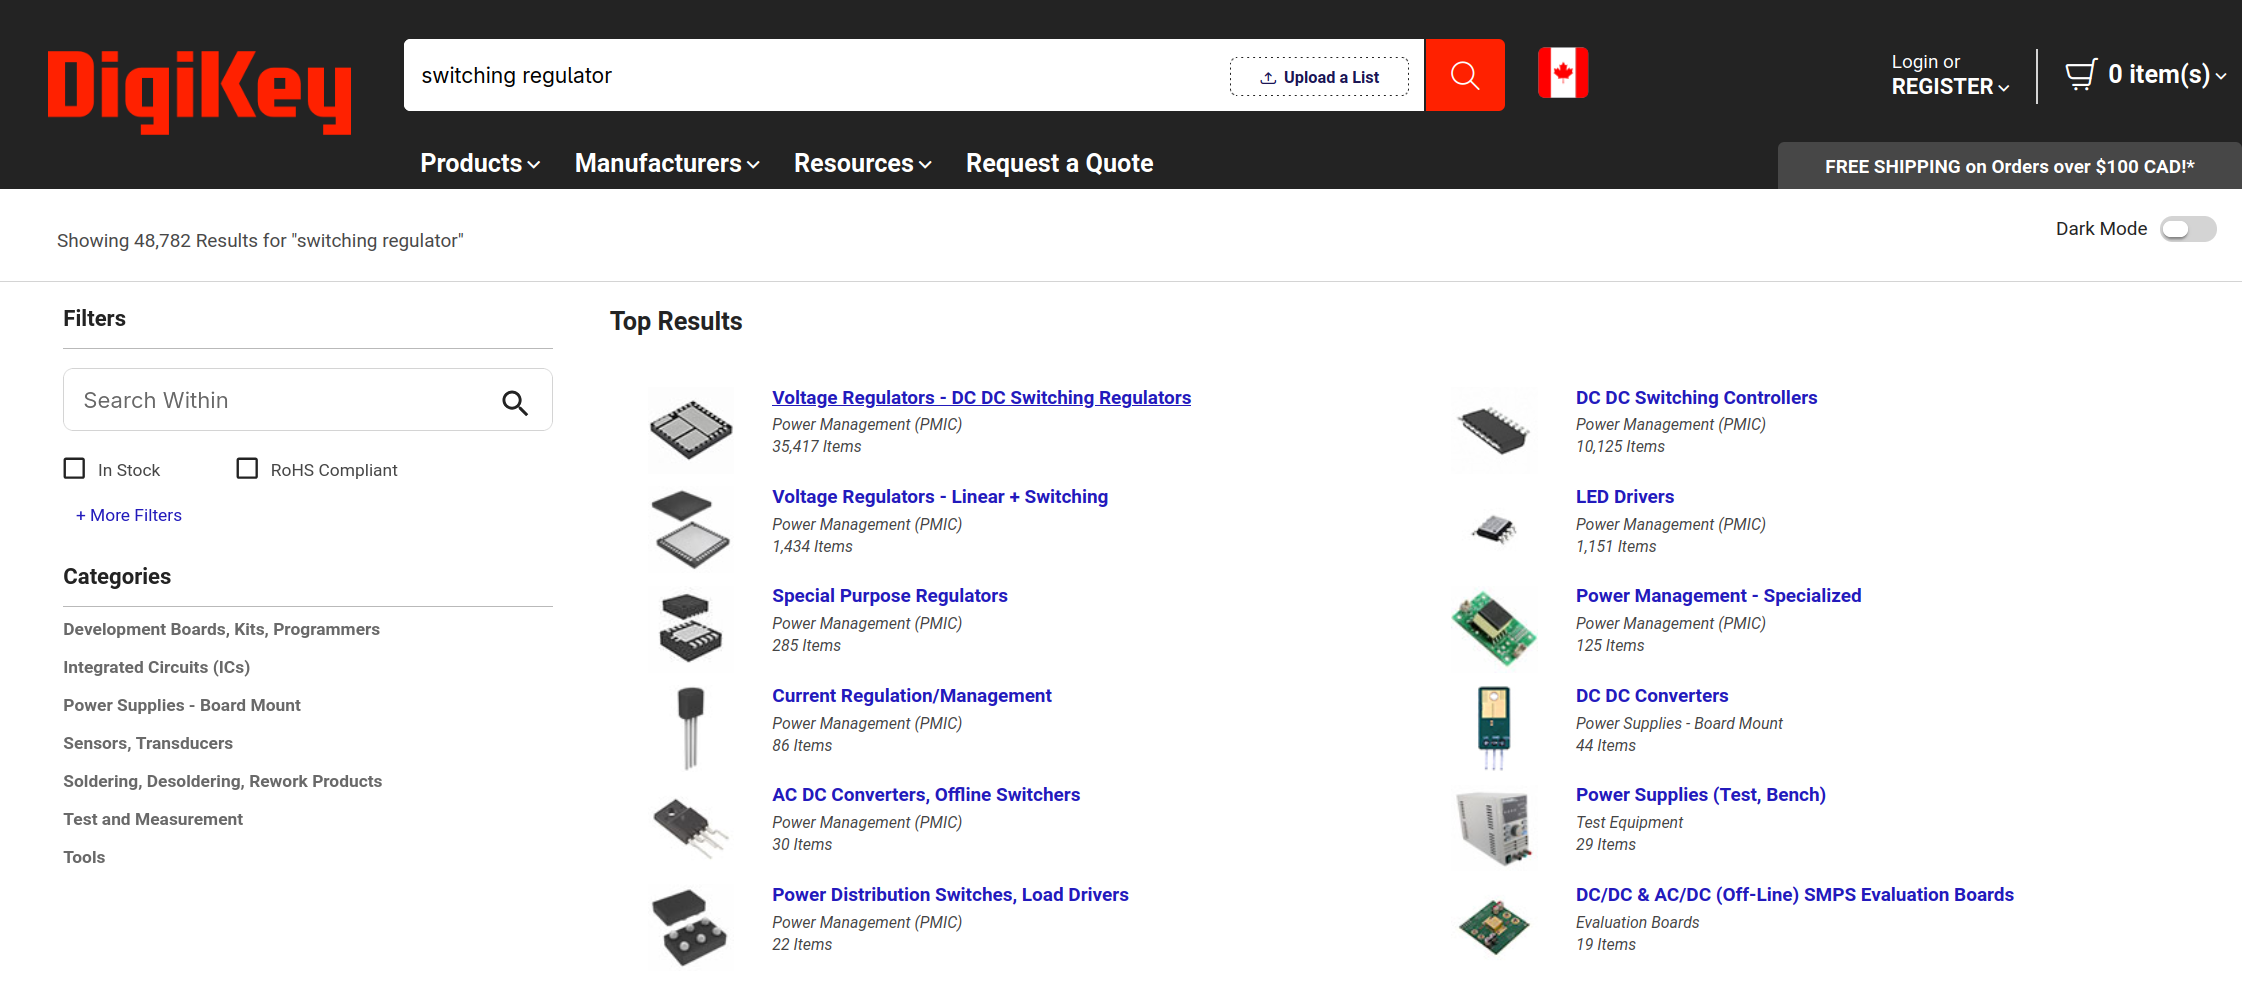
\includegraphics[width=\textwidth,
                                 height=0.9\textheight,
                                 keepaspectratio]{
                    pictures/digikey/search}
            };

            \draw[-Stealth, accent, ultra thick, rounded corners] (6.5, 6.2) -- (4.5, 6.2);
            \draw[-Stealth, accent, ultra thick, rounded corners] (8.25, 2.5) -- (7, 3.75);

            \node[circle, draw=accent, fill=white, inner sep=2pt, thick] at (7, 6.2) {1};
            \node[circle, draw=accent, fill=white, inner sep=2pt, thick] at (8.55, 2.2) {2};
        \end{tikzpicture}
    }
    \only<2>{
        \begin{tikzpicture}
            \node[anchor=south west, inner sep=0] at (0,0) {
                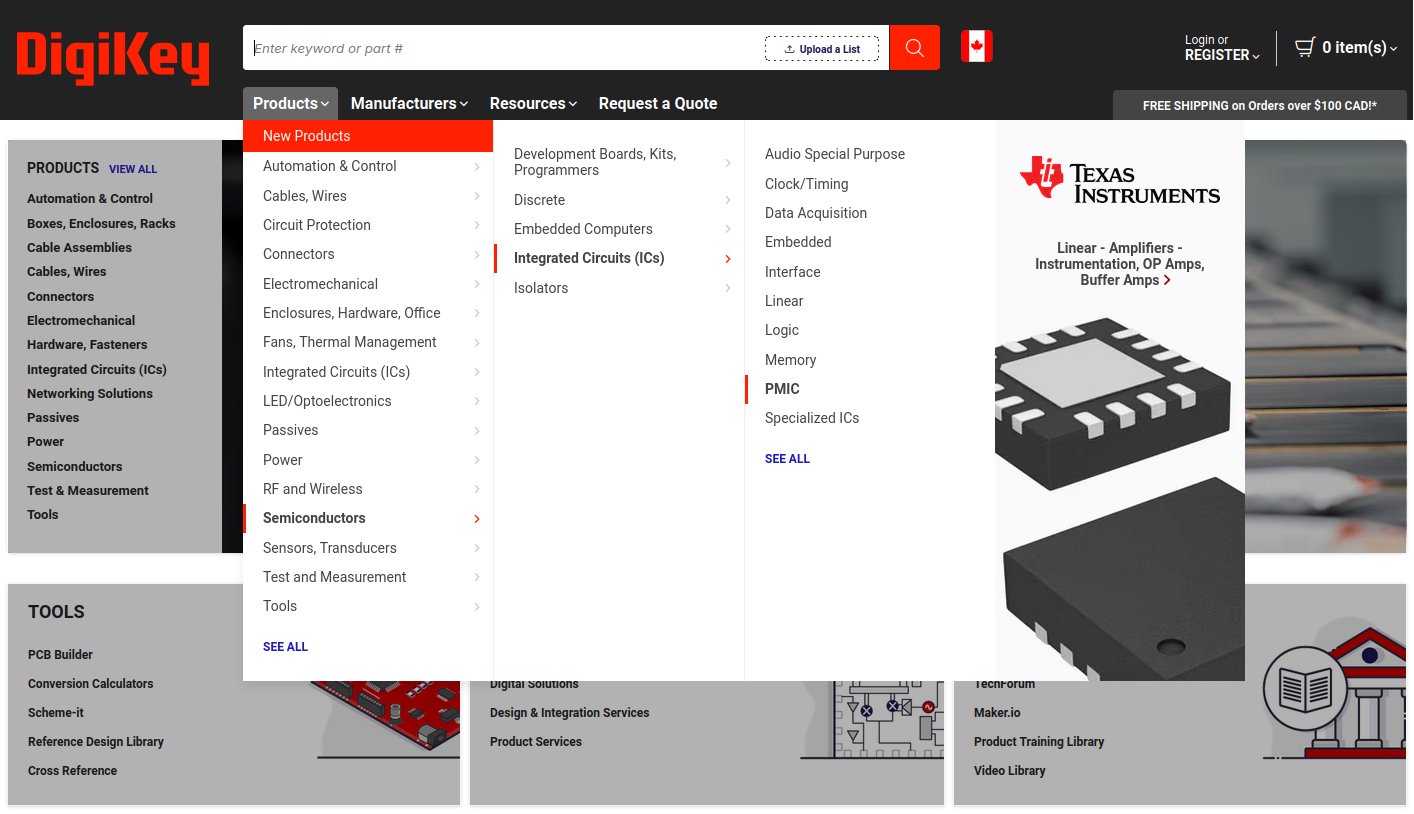
\includegraphics[width=\textwidth,
                                 height=0.8\textheight,
                                 keepaspectratio]{
                    pictures/digikey/main-page}
            };
 
            \draw[-Stealth, accent, very thick, rounded corners] (0.15, 6)   -- (2, 6);
            \draw[-Stealth, accent, very thick, rounded corners] (0.15, 2.45) -- (2, 2.45);
            \draw[-Stealth, accent, very thick, rounded corners] (2.4,  4.65) -- (4.1, 4.65);
            \draw[-Stealth, accent, very thick, rounded corners] (4.5,  3.58) -- (6.2, 3.58);

            \node[circle, draw=accent, fill=white, inner sep=2pt, thick] at (0.5, 6.4)  {1};
            \node[circle, draw=accent, fill=white, inner sep=2pt, thick] at (0.5, 2.85) {2};
            \node[circle, draw=accent, fill=white, inner sep=2pt, thick] at (1.9, 4.65) {3};
            \node[circle, draw=accent, fill=white, inner sep=2pt, thick] at (4,   3.58) {4};
        \end{tikzpicture}
    }
    \only<3-4>{
        \begin{tikzpicture}
            \node[anchor=south west, inner sep=0] (image) at (0,0) {
                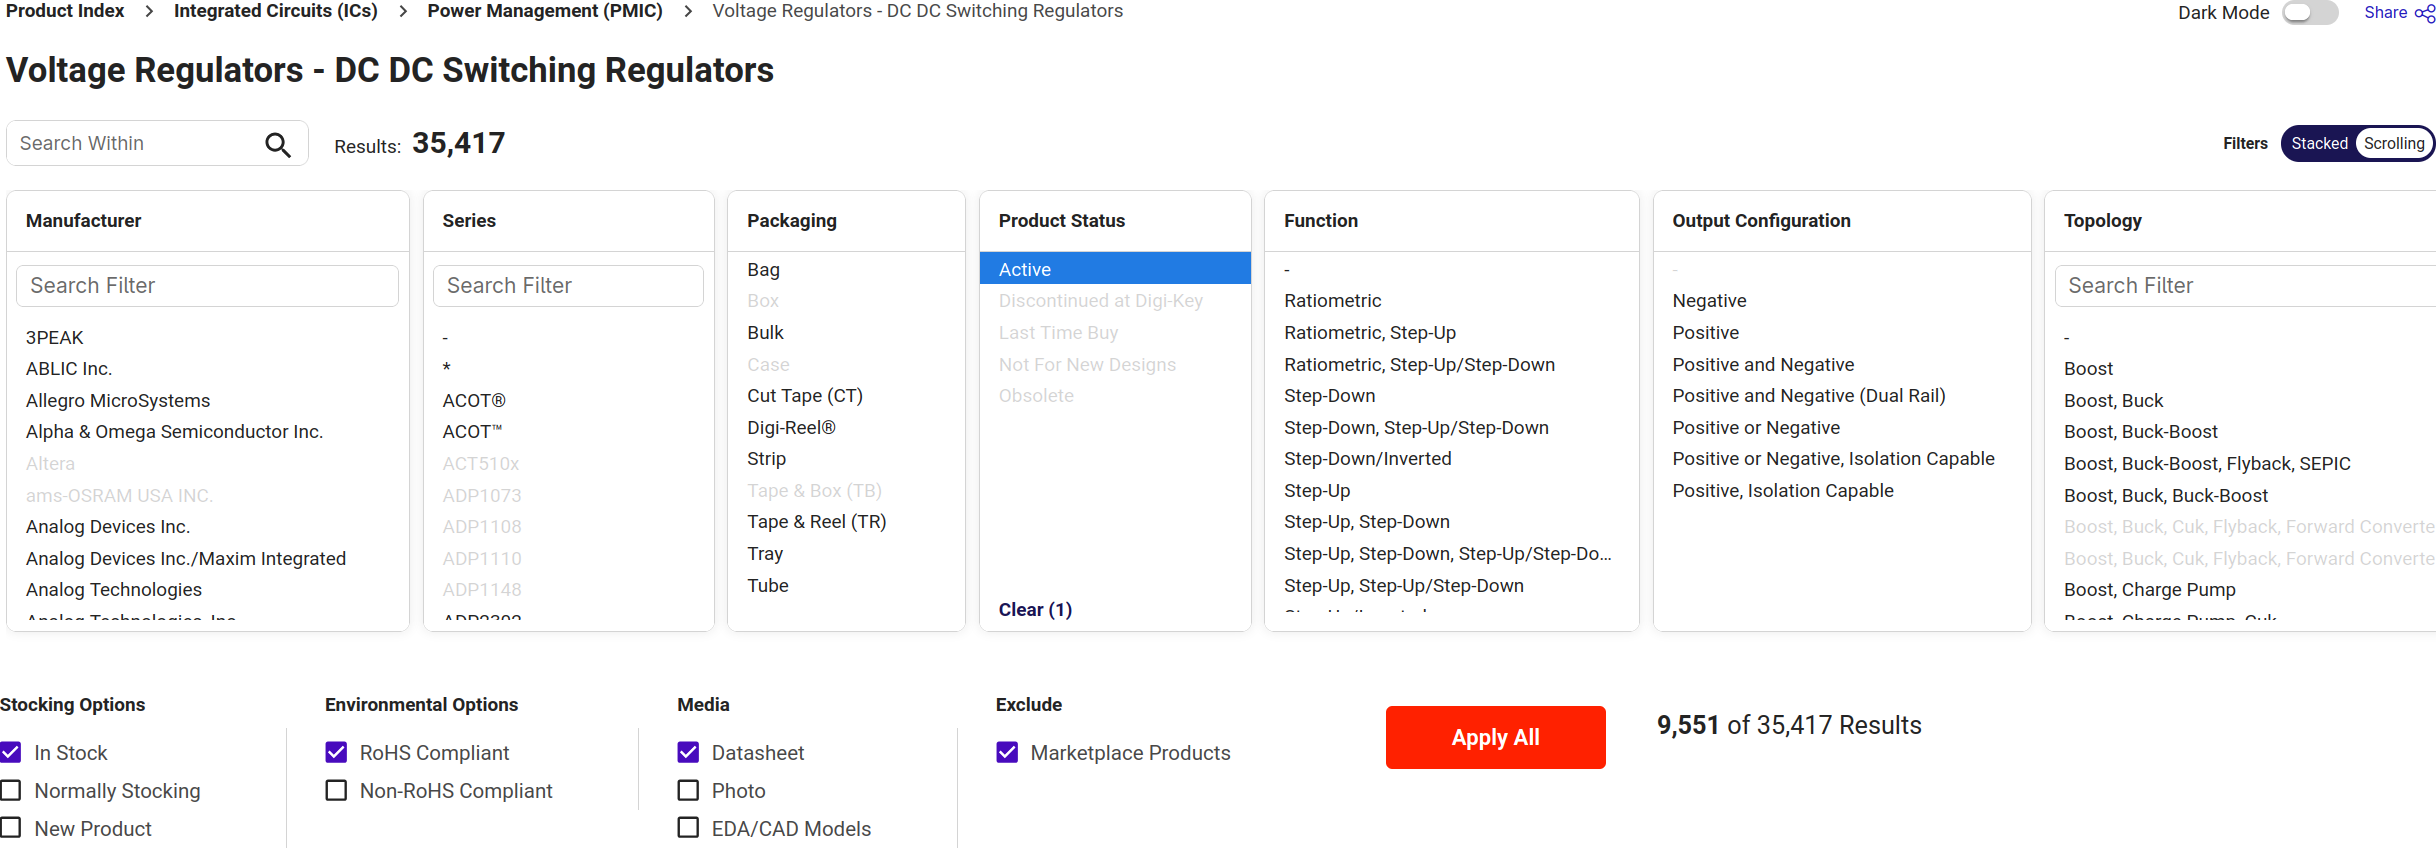
\includegraphics[width=\textwidth,
                                 height=0.9\textheight,
                                 keepaspectratio]{
                    pictures/digikey/first-filters}
            };
 
        \begin{scope}[x={(image.south east)}, y={(image.north west)}]
            \draw[-Stealth, accent, ultra thick, rounded corners] (0.08, 0)    -- (0.015, 0.09);
            \draw[-Stealth, accent, ultra thick, rounded corners] (0.2, 0)     -- (0.14, 0.09);
            \draw[-Stealth, accent, ultra thick, rounded corners] (0.2, 0.15) -- (0.27, 0.11);
            \draw[-Stealth, accent, ultra thick, rounded corners] (0.48, 0)    -- (0.425, 0.09);
            \draw[-Stealth, accent, ultra thick, rounded corners] (0.32, 0.68) -- (0.4, 0.68);

            \only<4> {
            \draw[-Stealth, accent2, ultra thick, rounded corners] (0.2, 0.04) -- (0.27, 0.02);
            %\node[circle, draw=accent2, fill=white, inner sep=2pt, thick] at (0.23, -0.05) {6};
            }

            %\node[circle, draw=accent, fill=white, inner sep=2pt, thick] at (0.07, 0.09) {1};
            %\node[circle, draw=accent, fill=white, inner sep=2pt, thick] at (0.16, -0.02) {2};
            %\node[circle, draw=accent, fill=white, inner sep=2pt, thick] at (0.23, 0.2)  {3};
            %\node[circle, draw=accent, fill=white, inner sep=2pt, thick] at (0.47, 0.09) {4};
            %\node[circle, draw=accent, fill=white, inner sep=2pt, thick] at (0.29, 0.68) {5};
        \end{scope}
        \end{tikzpicture}
    }
    \only<5>{
        \begin{tikzpicture}
            \node[anchor=south west, inner sep=0] (image) at (0,0) {
                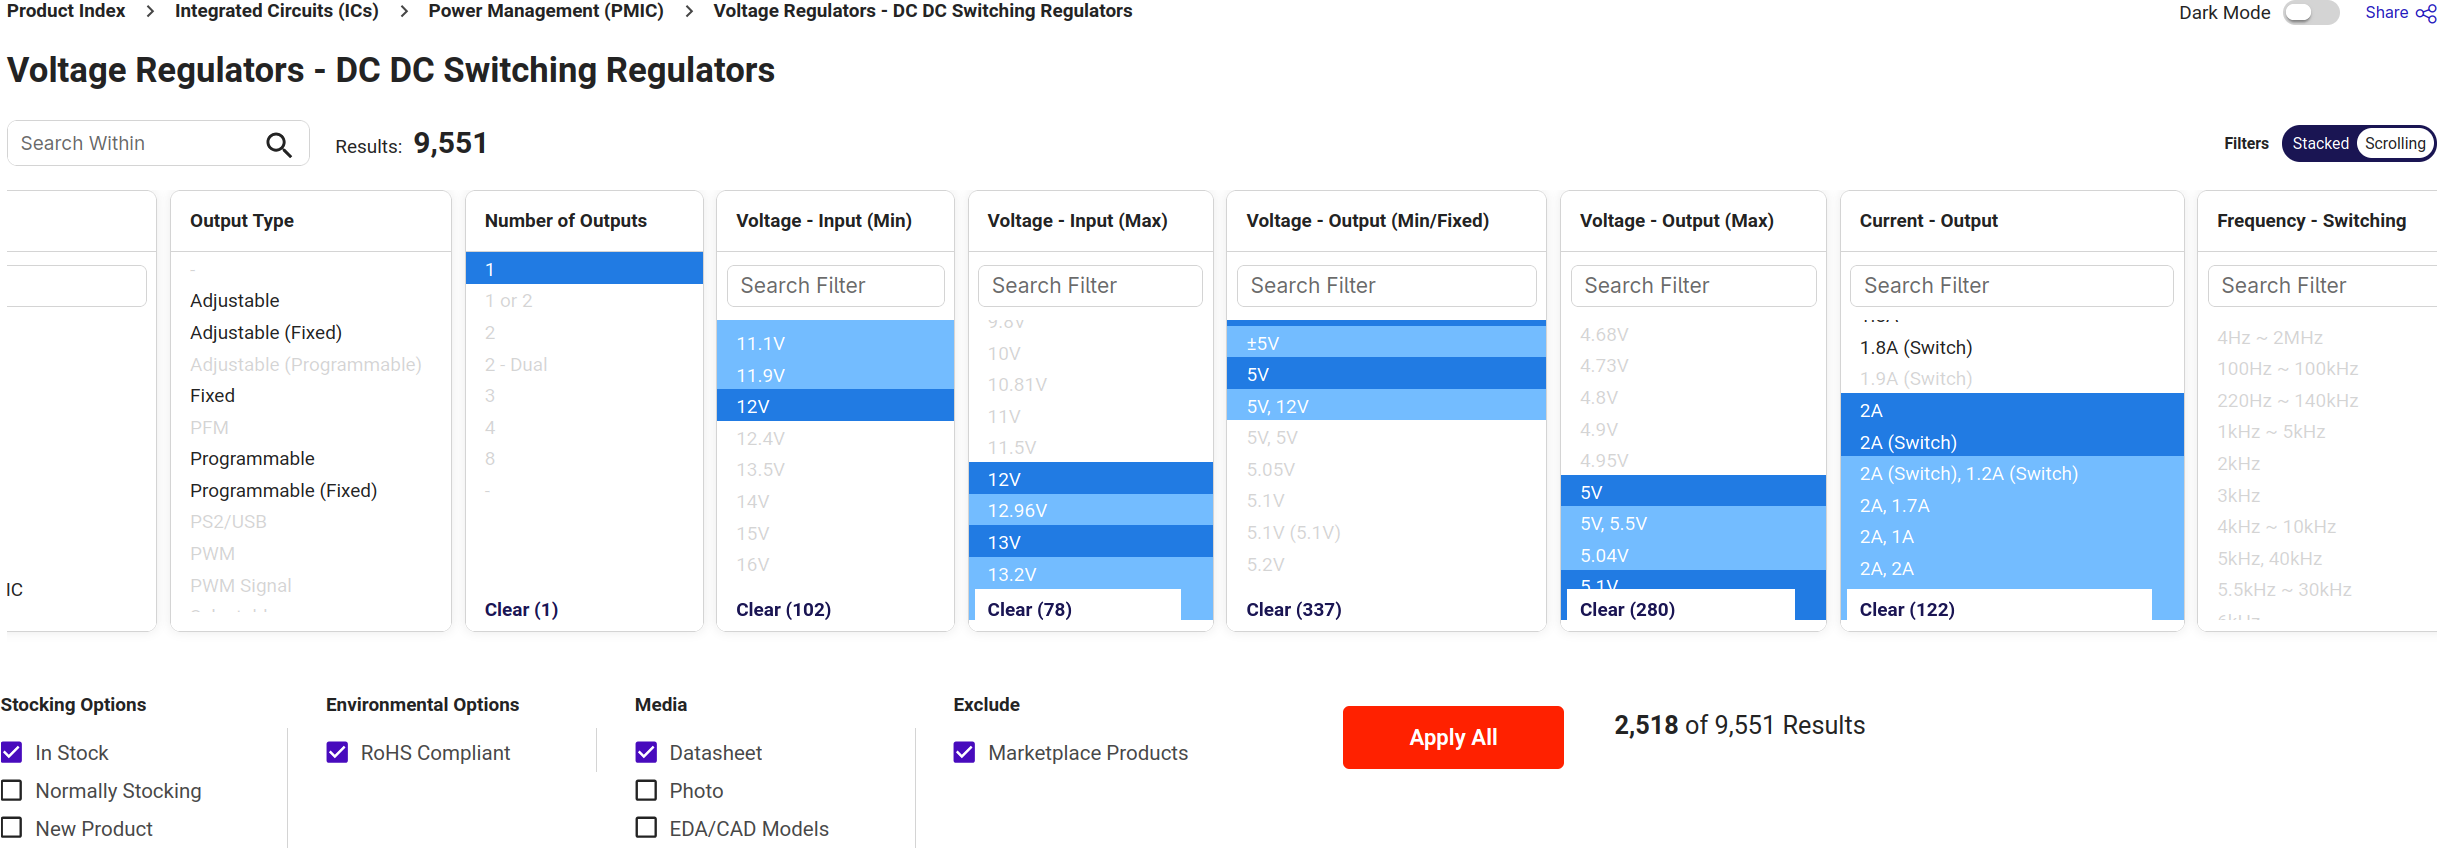
\includegraphics[width=\textwidth,
                                 height=0.9\textheight,
                                 keepaspectratio]{
                    pictures/digikey/power-filters}
            };
 
            \begin{scope}[x={(image.south east)}, y={(image.north west)}]
                \draw[-Stealth, accent, ultra thick, rounded corners] (0.1, 0.68)   -- (0.18, 0.68);
                \draw[-Stealth, accent, ultra thick, rounded corners] (0.34, 0.9)   -- (0.34, 0.65);
                \draw[-Stealth, accent, ultra thick, rounded corners] (0.44, 0)   -- (0.44, 0.2);
                \draw[-Stealth, accent, ultra thick, rounded corners] (0.56, 0.9)   -- (0.56, 0.65);
                \draw[-Stealth, accent, ultra thick, rounded corners] (0.69, 0)   -- (0.69, 0.2);
                \draw[-Stealth, accent, ultra thick, rounded corners] (0.82, 0)   -- (0.82, 0.2);
            \end{scope}
        \end{tikzpicture}
    }
    \only<6>{
        \begin{tikzpicture}
            \node[anchor=south west, inner sep=0] (image) at (0,0) {
                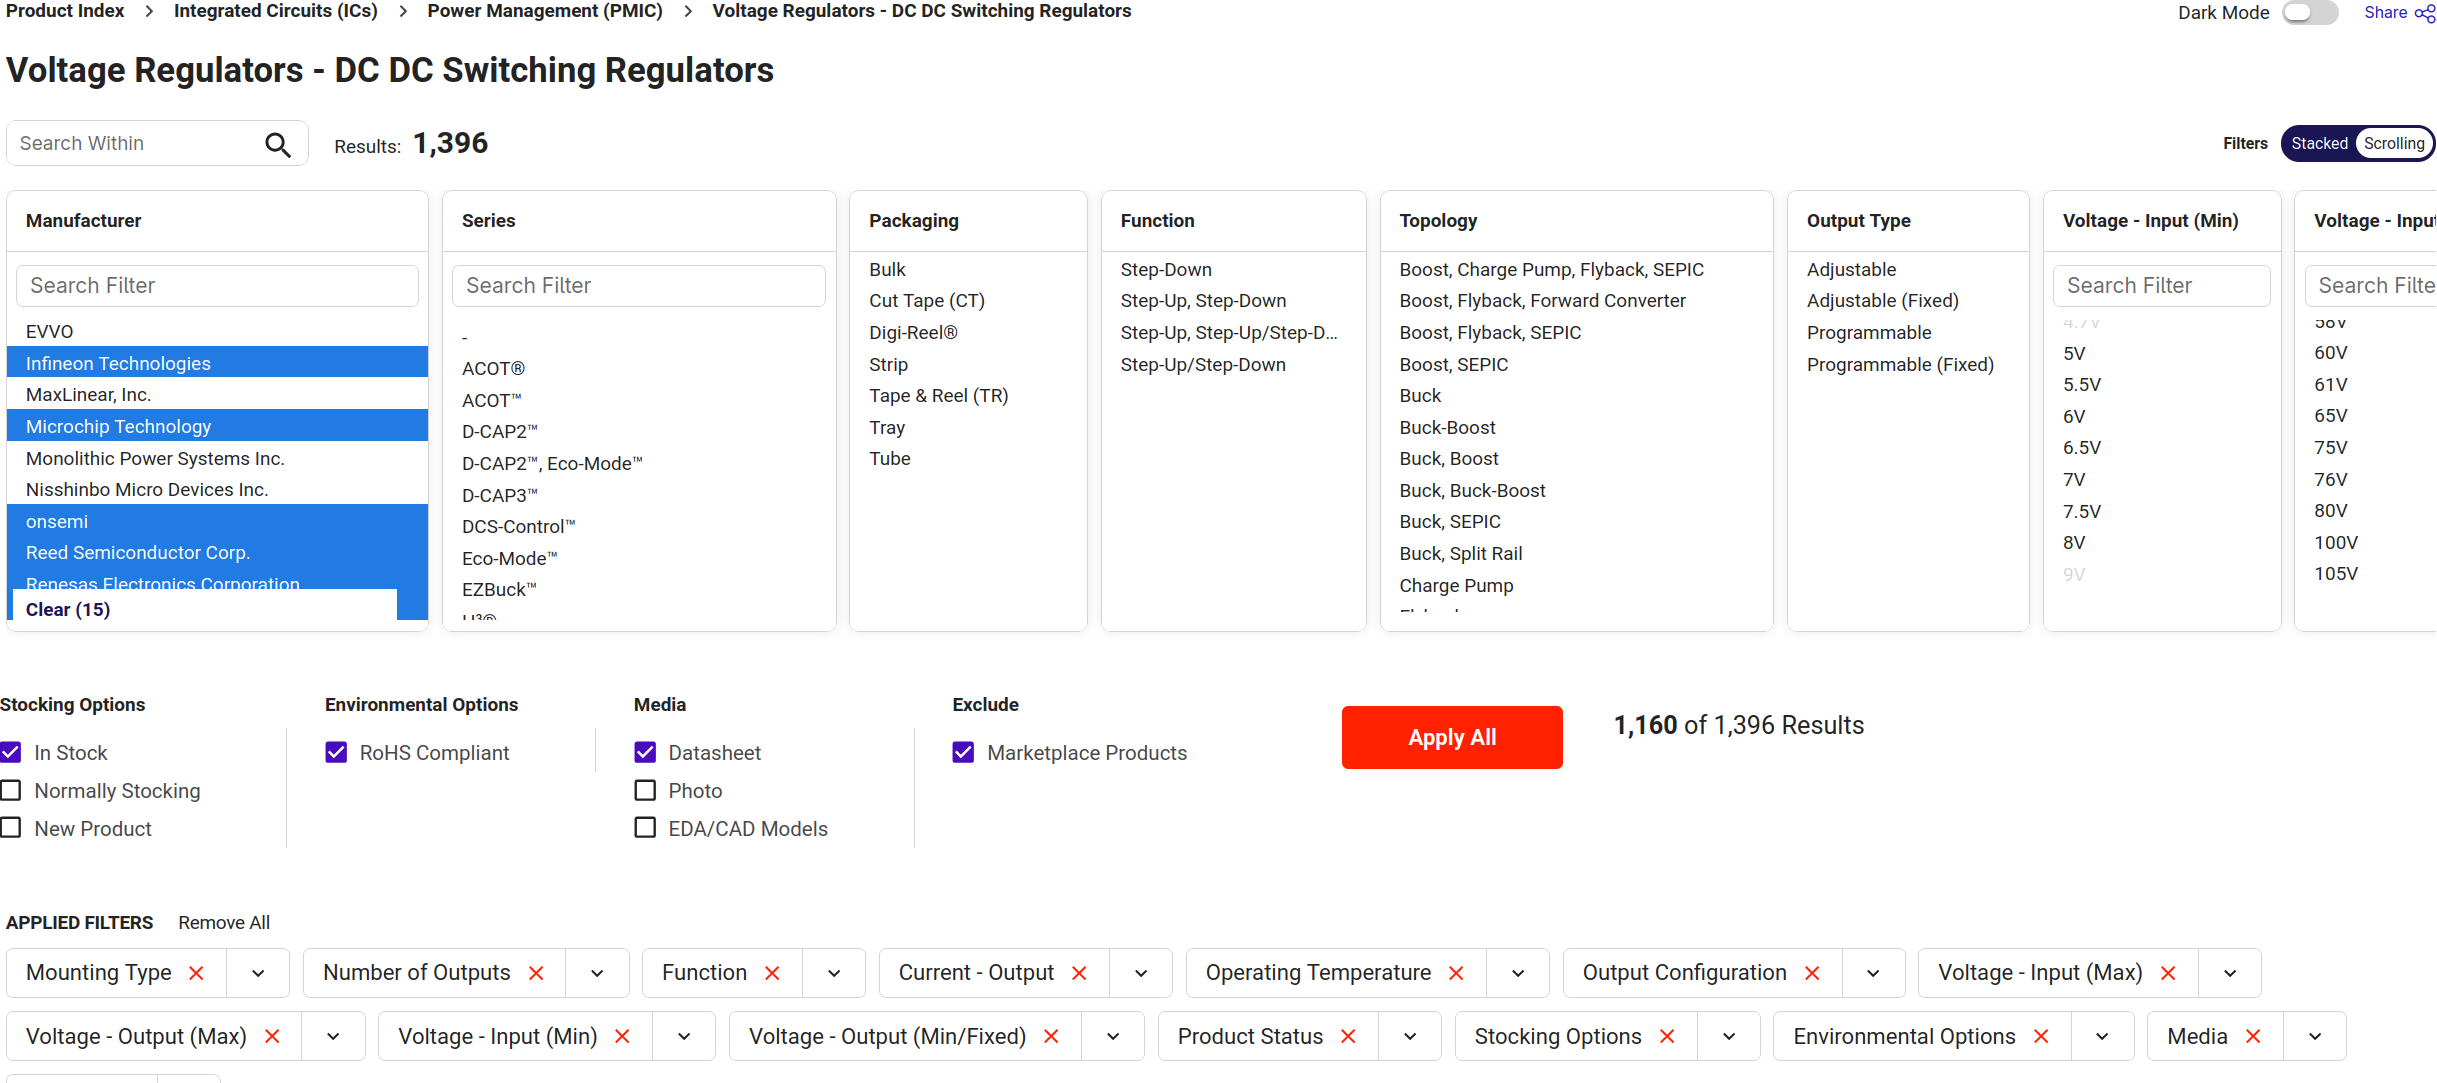
\includegraphics[width=\textwidth,
                                 height=0.9\textheight,
                                 keepaspectratio]{
                    pictures/digikey/mfr-filters}
            };
 
            \begin{scope}[x={(image.south east)}, y={(image.north west)}]
                \draw[-Stealth, accent, ultra thick, rounded corners] (0.08, 0.9)   -- (0.08, 0.725);
            \end{scope}
        \end{tikzpicture}
    }
    \only<7>{
        \begin{tikzpicture}
            \node[anchor=south west, inner sep=0] (image) at (0,0) {
                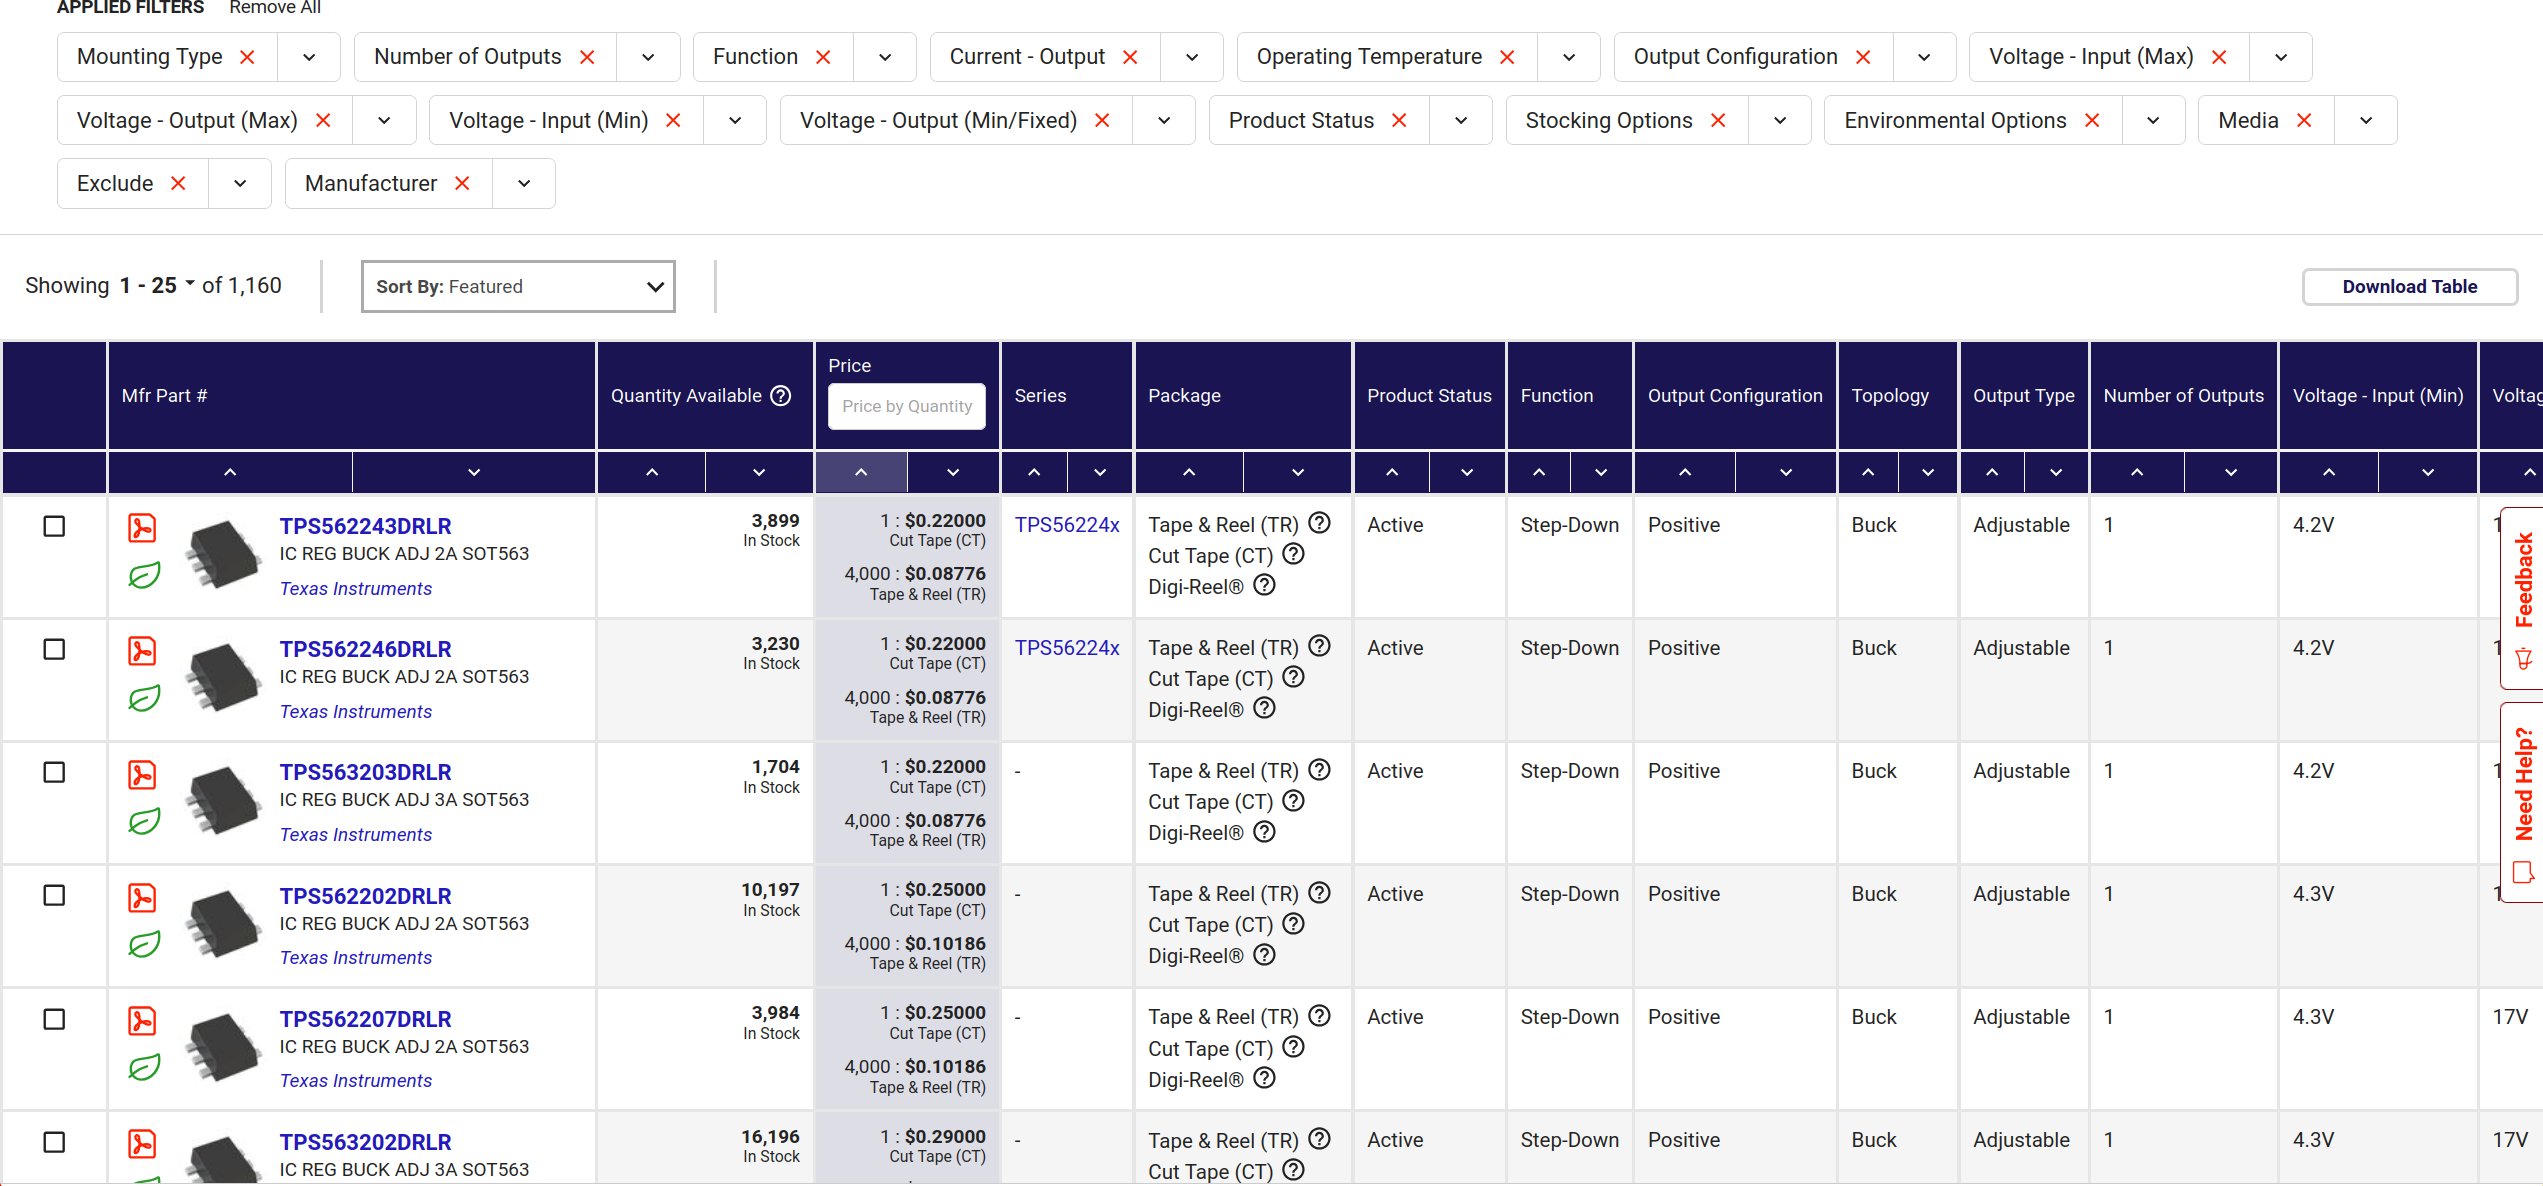
\includegraphics[width=\textwidth,
                                 height=0.8\textheight,
                                 keepaspectratio]{
                    pictures/digikey/ordering}
            };
 
            \begin{scope}[x={(image.south east)}, y={(image.north west)}]
                \draw[-Stealth, accent, ultra thick, rounded corners] (0.3, 0.75)   -- (0.335, 0.62);
            \end{scope}
        \end{tikzpicture}
    }
    \only<8>{
        \begin{twocolumns}
            \leftcol
            \makefigure[1][0.8]{digikey/tps562243}
            \rightcol
            \makefigure[1][0.8]{digikey/tps562243-datasheet}
        \end{twocolumns}
    }
    \only<9>{
        \makefigure[1][0.8]{digikey/tps562243-uvlo}
    }
    \only<10>{
        \begin{twocolumns}
            \leftcol
            \makefigure[1][0.8]{digikey/bd95841}
            \rightcol
            \makefigure[1][0.8]{digikey/bd95841-datasheet}
        \end{twocolumns}
    }
    \end{center}
\end{frame}

\subsection{BOM}

\begin{frame}{Erreurs communes dans un BOM}
    \begin{twocolumns}[0.33]
        \leftcol
        \begin{itemize}
            \item Erreurs de copier-coller
            \item Items manquants
            \item Mauvaise pièce commandée
        \end{itemize}

        \rightcol
        \centering
        \only<2->{
            \begin{tabular}{l | c | c}
                \textbf{Designators} & \textbf{Value} & \textbf{Footprint}\\
                \hline
                C1, C3, C4, C5, C9 & $\SI{10}{\micro\farad}$ & 1206\\
                C2, C7, C8, C11    & $\SI{100}{\nano\farad}$ & 0402\\
                C6                 & $\SI{10}{\micro\farad}$ & \textcolor{red}{1206}\\
            \end{tabular}\\
            \vspace{24pt}
            \begin{tabular}{l | l}
                \textbf{Designators} & \textbf{Description}\\
                \hline
                F1 & Fuse Holderr\\
                \textcolor{red}{\st{F2}} & \textcolor{red}{\st{Fuse 2A}}\\
            \end{tabular}\\
            \vspace{24pt}
            \begin{tabular}{c | l | l}
                \textbf{Designators} & \textbf{Description} & \textbf{Part number}\\
                \hline
                U1 & Régulateur 1.8V & AP2120N-3.3TRG1\\
            \end{tabular}
        }
    \end{twocolumns}
\end{frame}

\begin{frame}{Éviter des erreurs de copier-coller}
    \begin{itemize}
        \item Se faire une page avec une liste des composantes passives utilisées
        \item Retourner à la page et copier la composante désirée
    \end{itemize}

    \makefigure[1][0.66]{bom-component-list}
\end{frame}

\begin{frame}{Éviter des erreurs de copier-coller}
    \begin{itemize}
        \item Créer une librairie spécifique au projet
        \item Créer des symboles spécifiques pour toutes les composantes passives
        \item Pas besoin de page bizarre ou de fignolage avec les options
        \bigskip
        \item Dans les deux cas:
        \begin{itemize}
            \item Choisir des modèles de passives dès le début du projet
        \end{itemize}
    \end{itemize}
\end{frame}

\begin{frame}{Quoi mettre dans un BOM}
    \begin{twocolumns}
        \leftcol
        \begin{itemize}
            \item Tout ce qui fait partie d'un assemblage
            \item Pas juste ce qui va directement sur le PCB
        \end{itemize}

        \footnotesize
        \begin{columns}
            \begin{column}{0.05\textwidth}
            \end{column}
            \begin{column}{0.95\textwidth}
                \begin{itemize}
                    \item Vis, standoffs, washers
                    \item Câbles, alimentations, boîtiers
                    \item Fusibles, connecteurs, écrans, jumpers
                    \item Stencils, pâte, heatsinks
                \end{itemize}
            \end{column}
        \end{columns}
        \rightcol
        \makefigure[1][0.35]{bom-wall-adapter}
    \end{twocolumns}
    
    \begin{columns}
        \begin{column}{0.33\textwidth}
            \makefigure[1][0.33]{bom-fuse}
        \end{column}
        \begin{column}{0.33\textwidth}
            \makefigure[1][0.33]{bom-jumper}
        \end{column}
        \begin{column}{0.33\textwidth}
            \makefigure[1][0.35]{bom-screws}
        \end{column}
    \end{columns}
\end{frame}

\begin{frame}{Révision du BOM}
    \begin{itemize}
        \item Plusieurs personnes impliquées
        \begin{itemize}
            \item Achats
            \item Assemblage du PCB
            \item Assemblage du produit
            \item Debugging
        \end{itemize}
        \bigskip
        \item Valider qu'il y a tout ce qu'il faut acheter
        \item Valider qu'il ne manque rien
        \item Valider que toutes les composantes font du sens
        \item Valider qu'il n'y a pas d'incompatibilité
        \item Valider que les part\,\# matchent
    \end{itemize}
\end{frame}

\begin{frame}{Coûts -- Règles du pouce}
    \begin{twocolumns}[0.55]
        \leftcol
        \centering
        \textbf{Un assemblage va coûter environ autant que les pièces}

        \rightcol
        \centering
        \textbf{Ton coût de vente devrait être 2.5× ton coût de production}\\
        Source: \cite{eevblog-economics}
    \end{twocolumns}

    \begin{twocolumns}[0.555]
        \leftcol
        \begin{itemize}
            \item Pièces plus petites ont besoin de procédés avancés
            \begin{itemize}
                \item BGA
                \item Small-pitch
                \item 0201
            \end{itemize}
            \item Pièces complexes = assemblages complexes
            \begin{itemize}
                \item Heatsinks et pâte thermique
                \item Shielding EMI
                \item Connecteurs funky
                \item Pogo pins
            \end{itemize}
            \item Beaucoup de pièces = + passages dans la PnP
            \item Courbes de températures spécifiques
        \end{itemize}

        \rightcol
        \begin{itemize}
            \item Frais de shipping, packaging, retour
            \item Yield et testing
            \item Distributeurs veulent une part du profit
            \bigskip
            \item Il faut tirer un profit assez gros pour être sustenable
            \item Il faut tirer un profit assez gros pour que ça vaille la peine
        \end{itemize}
    \end{twocolumns}
\end{frame}

\begin{frame}{Consolidation du BOM}
    \begin{itemize}
        \item On veut donc \textit{diminuer la taille du BOM}
        \item Nombre de pièces limitées dans la PnP ($\sim 48$ dans la PnP du 3iT)
        \item Chaque pièce est commandée en quantité minimum
        \item Gaspillage + Augmenter complexité assemblage
        \bigskip
        \item Il faut donc \textbf{consolider} le BOM
    \end{itemize}
\end{frame}

\begin{frame}{Consolidation du BOM}
    \begin{columns}
        \begin{column}{0.05\textwidth}
        \end{column}
        \begin{column}{0.5\textwidth}
            \begin{centering}
            \textbf{Minimum Order Quantity: 70}\\
            \end{centering}
            \vspace{12pt}
            \begin{tabular}{c | c | c | c | c}
                \textbf{Value} & \textbf{Qty} & \textbf{Cost} & \textbf{Total} & \textbf{Real Total}\\
                \hline
                $\SI{1}{\kilo\ohm}$ & 20 & 2¢ & 40¢ & 1.4\$\\
                $\SI{2}{\kilo\ohm}$ & 1  & 2¢ & 2¢  & 1.4\$\\
                \textbf{Total}      &    &    &     & 2.8\$
            \end{tabular}

            \vspace{24pt}

            \only<1>{
                \begin{itemize}
                    \item Les minimum order quantity peuvent affecter le prix
                    \item Une seule résistance peut en valoir 70
                    \bigskip
                    \item Combiner des résistances en série ou parallèle!
                \end{itemize}
            }
            \only<2>{
            \begin{tabular}{c | c | c | c | c}
                \textbf{Value} & \textbf{Qty} & \textbf{Cost} & \textbf{Total} & \textbf{Real Total}\\
                \hline
                $\SI{1}{\kilo\ohm}$ & 22 & 2¢ & 44¢ & 1.4\$\\
                \textbf{Total}      &    &    &     & 1.4\$
            \end{tabular}
            }

        \end{column}
        \begin{column}{0.25\textwidth}
            \begin{maketikzfigure}
                \node[vcc] at (0, 0) {};

                \draw (0, 0)
                to [R, l=$\SI{1}{\kilo\ohm}$] (0, -2)
                to [short, -*] (1, -2);

                \only<1>{
                    \draw (0, -2)
                    to [R, l=$\SI{2}{\kilo\ohm}$] (0, -4)
                    to node[ground]{} (0, -4);
                }
                \only<2>{
                    \draw (0, -2)
                    to [R, l=$\SI{2}{\kilo\ohm}$, color=accent2] (0, -4)
                    to node[ground]{} (0, -4);
                }
            \end{maketikzfigure}
        \end{column}

        \begin{column}{0.25\textwidth}
            \only<2>{
            \begin{maketikzfigure}
                \node[vcc] at (0, 0) {};

                \draw (0, 0)
                to [R, l=$\SI{1}{\kilo\ohm}$] (0, -2)
                to [short, -*] (1, -2);
                \draw (0, -2)
                to [R, l=$\SI{1}{\kilo\ohm}$, color=accent] (0, -4)
                to [R, l=$\SI{1}{\kilo\ohm}$, color=accent] (0, -6)
                to node[ground]{} (0, -6);
            \end{maketikzfigure}
            }
        \end{column}
    \end{columns}
\end{frame}

\begin{frame}{Consolidation du BOM}
    \textbf{Minimum Order Quantity: 70}\\
    \vspace{12pt}
    \begin{tabular}{m{12em} | c | c | c | c | c | c}
        \textbf{Designators} & \textbf{Value} & \textbf{Footprint} & \textbf{Qty} & \textbf{Cost} & \textbf{Total} & \textbf{Real Total}\\
        \hline
        C14, C15, C16, C17 & $\SI{1}{\micro\farad}$ & 0603 & 4 & 10¢ & 40¢ & 7\$\\
        C25, C26, C27, C28 & $\SI{1}{\micro\farad}$ & 1206 & 4 & 1¢  & 4¢  & 70¢\\
        \textbf{Total}     &                        &      &   &     &     & 7.7\$
    \end{tabular}

    \vspace{24pt}

    \only<1>{
        \begin{itemize}
            \item C25, C26, C27 \& C28 sont des condensateurs gros et cheap
            \item C14, C15, C16 \& C17 sont des condensateurs plus chers
            \bigskip
            \item On a besoin des caractéristiques de ces condensateurs plus chers dans une section
            \item Dans des faibles quantités d'assemblage, il peut être mieux d'acheter juste des condensateurs chers
        \end{itemize}
    }

    \only<2>{
    \begin{tabular}{m{12em} | c | c | c | c | c | c}
        \textbf{Designators} & \textbf{Value} & \textbf{Footprint} & \textbf{Qty} & \textbf{Cost} & \textbf{Total} & \textbf{Real Total}\\
        \hline
        C14, C15, C16, C17, C25 & $\SI{1}{\micro\farad}$ & 0603 & 5 & 10¢ & 50¢ & 7\$\\
        \textbf{Total}          &                        &      &   &     &     & 7\$
    \end{tabular}
    }
\end{frame}

\begin{frame}{Quand utiliser des pièces qui coûtent cher?}
    \vspace{-6pt}
    \begin{center}
        \begin{tabular}{c | c | c | c | c | c}
            \textbf{Part Number} & \textbf{Type} & \textbf{Voltage} & \textbf{Tolérance} & \textbf{Ratings} & \textbf{Coût/100}\\
            \hline
            CGA2B3X7R1H473K050EB & X7R           & $\SI{50}{\volt}$ & 10\% & AEC-Q200 & 2.94\$\\
            GRM155R71E473KA88D   & X7R           & $\SI{16}{\volt}$ & 20\% & --       & 1.86\$\\
        \end{tabular}\\
        \vspace{6pt}
        \textbf{On PCB: 10}\\
        \textbf{Minimum Order Quantity: 100}\\
        \vspace{-6pt}
    \end{center}
    \begin{twocolumns}
        \leftcol
        \begin{center}
            \textbf{2 Million / année}\\
        \end{center}
        \rightcol
        \begin{center}
            \textbf{2 prototypes pour l'uni}\\
        \end{center}
    \end{twocolumns}
    \pause
    \begin{twocolumns}
        \leftcol
        \textbf{Option 1:}\\
        \begin{center}
            $\frac{2.94\$}{100} \cdot 10 \cdot 2\,000\,000 = 588\,000\$$\\
        \end{center}

        \textbf{Option 2:}\\
        \begin{center}
            $\frac{1.86\$}{100} \cdot 10 \cdot 2\,000\,000 = 372\,000\$$\\
        \end{center}

        \begin{center}
        $588\,000\$ - 372\,000\$ = 216\,000\$$
        \end{center}

        \rightcol
        Commande = quantité minimale\\

        \textbf{Option 1:} $2.94\$$\\
        \textbf{Option 2:} $1.86\$$\\

        \begin{center}
        $2.94\$ - 1.86\$ = 1.08\$$
        \end{center}

    \end{twocolumns}
\end{frame}
